\chapter{Results}    \label{results}
\section{Recruitment of Rvs to endocytic sites}

Rvs localization in yeast endocytosis
As has been shown before, Rvs localizes to endocytic patches at the yeast plasma membrane in the late scission-stage8,9. When imaged and tracked at the equatorial plane, the late-stage coat protein Sla1 arrives and accumulates at endocytic sites, starts to moves into the cytoplasm concomitant with the arrival of actin8,9. Sla1 is pulled inwards along with the membrane and follows its movement through endocytosis. It will be used throughout this work as the marker for coat movement. As inward movement of the coat begins, the Sla1 patch is disassembled, inferred from the decay of the fluorescent intensity of Sla1-GFP8. Rvs167 arrives after a parallel membrane tube is formed, and scission occurs at 60\% of its lifetime at the plasma membrane9,10. At the time of scission, the Rvs167-GFP centroid shows a sharp jump into the cytoplasm, a profile that is unique among endocytic proteins. Concomitantly, fluorescent intensity of Rvs167-GFP shows a sudden decay.

\begin{figure}
	\centering
	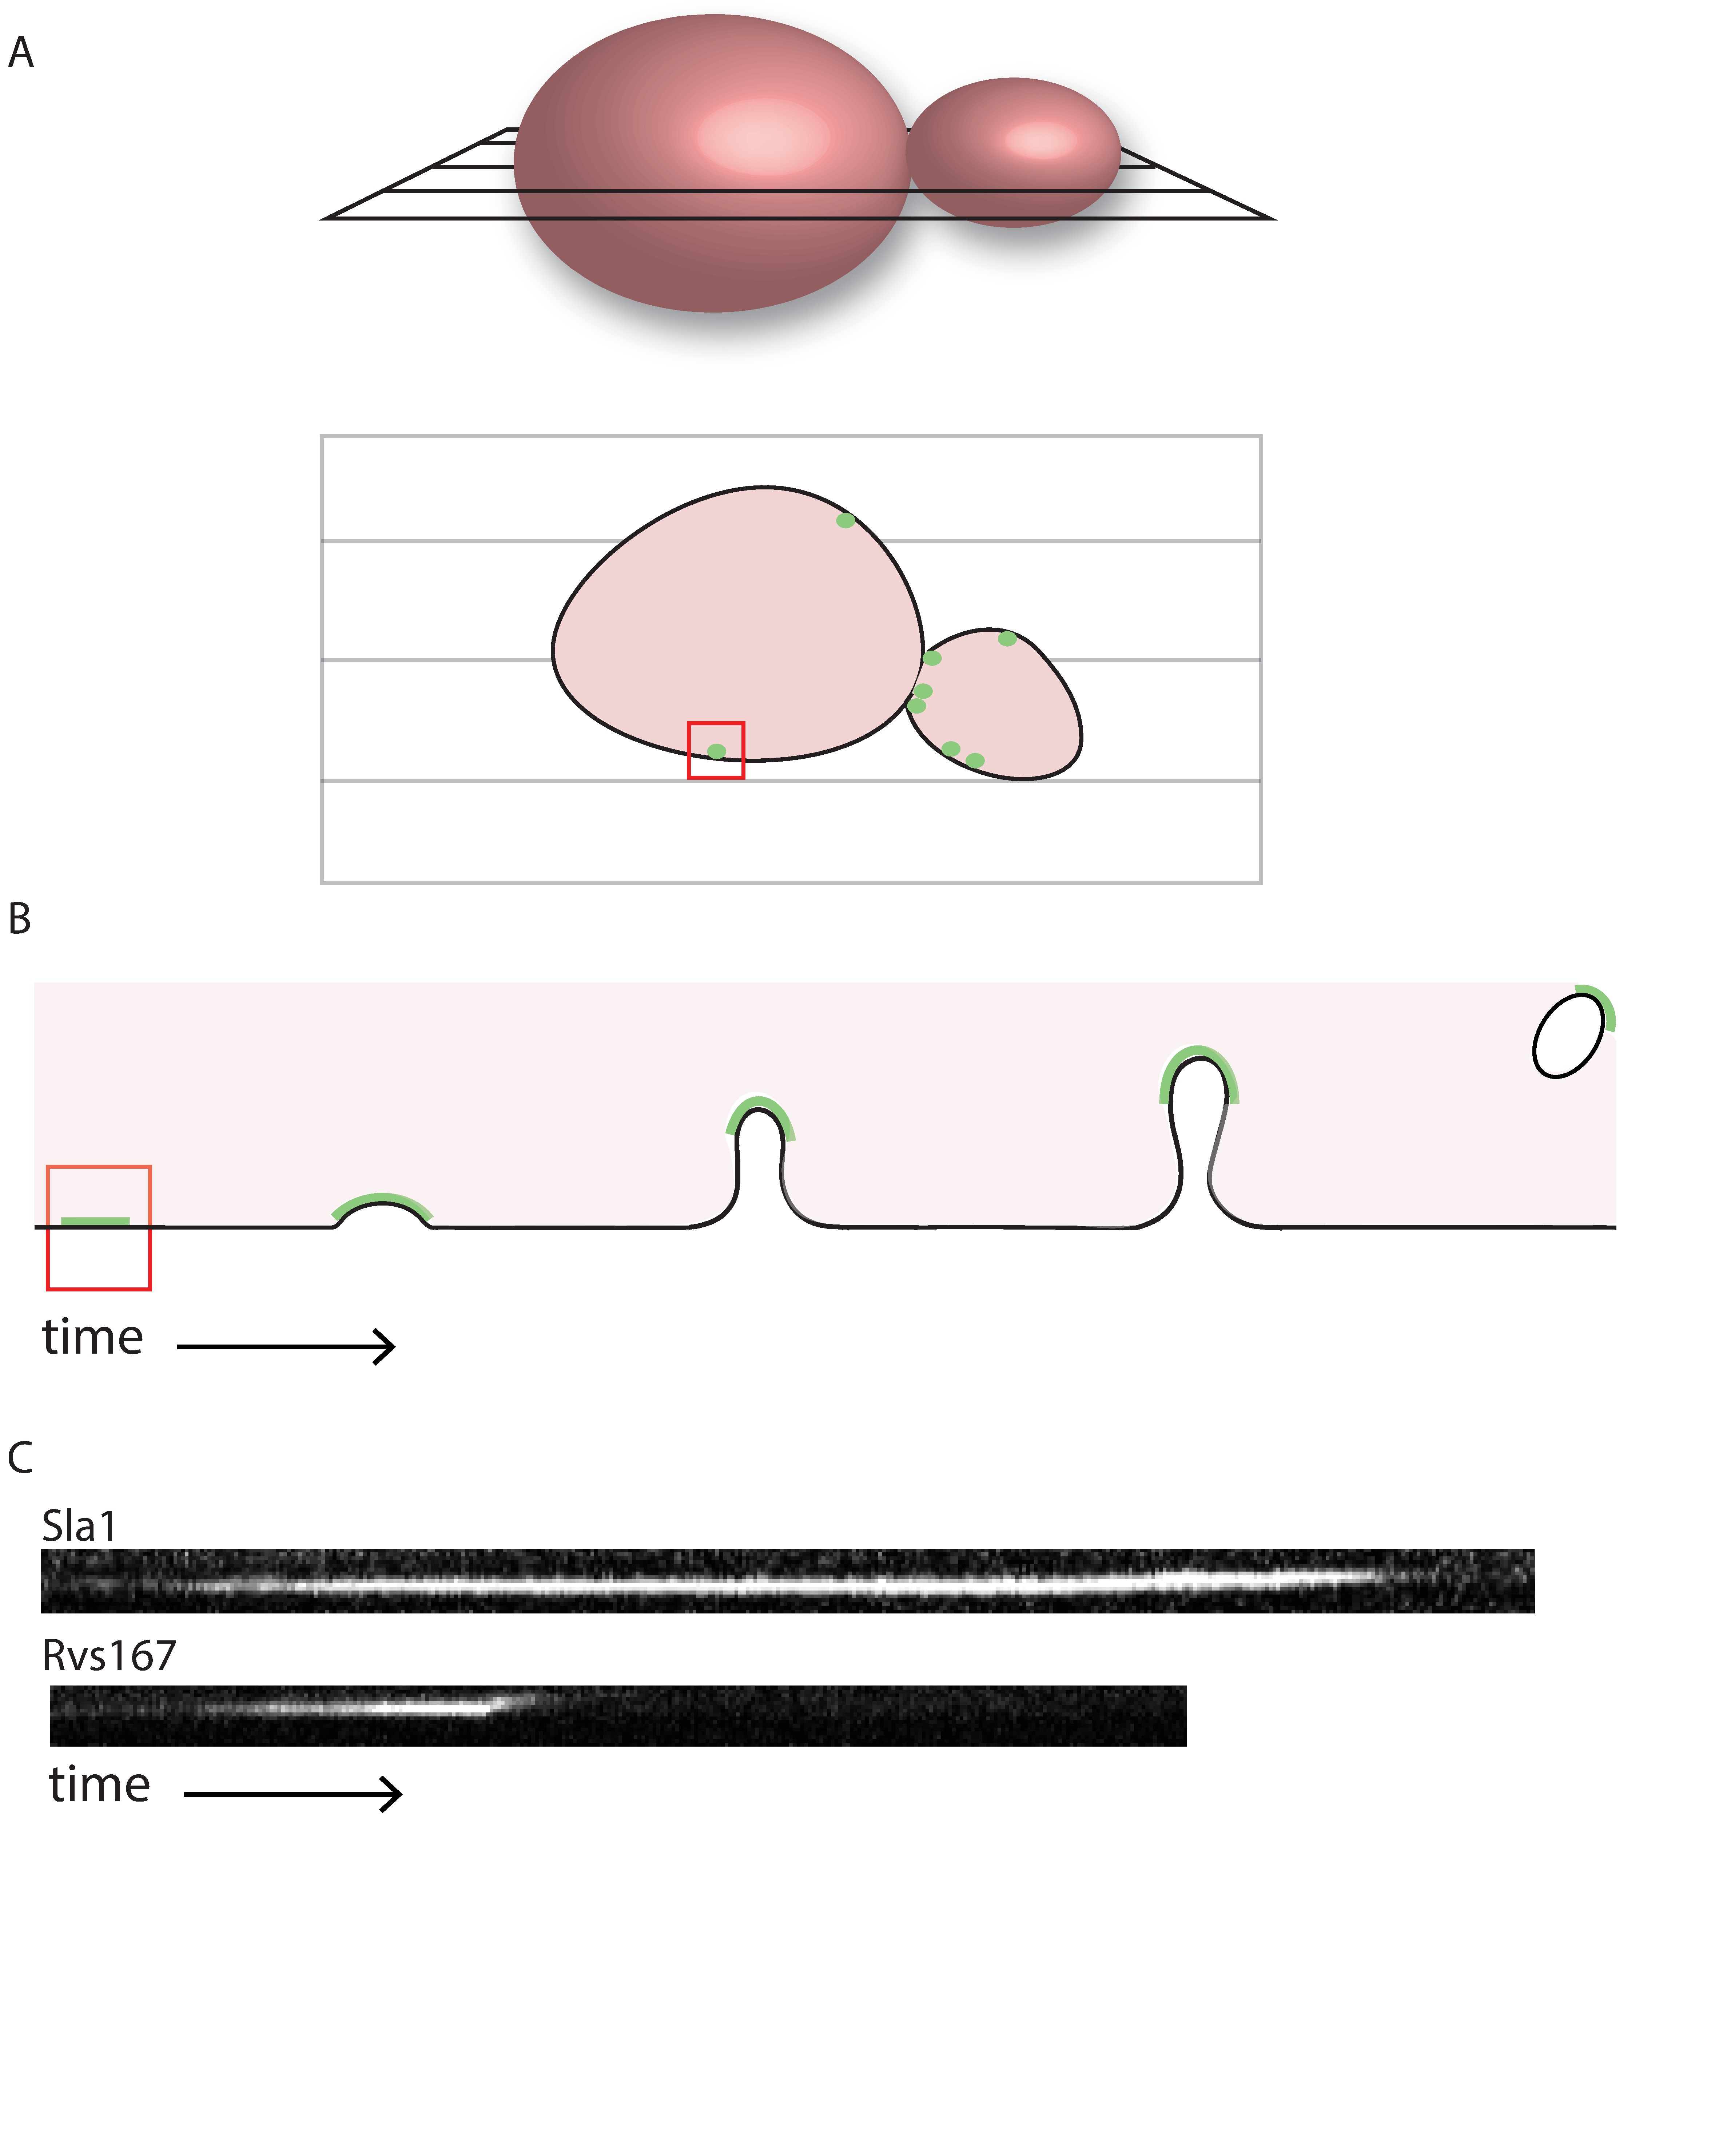
\includegraphics[width=18cm,height=18cm,keepaspectratio, valign=t]{figures/results_final/yeast_schemat_fig1_C}
	\caption[Centroid tracking yeast endocytic proteins]
	{A: Above: Schematic of a yeast cell, showing the equatorial plane. Below: Cross section of the cell at the equatorial plane, with fluorescently tagged endocytic proteins at the plasma membrane. B: Movement of coat protein Sla1-GFP shows slow inward movement, while Rvs167-GFP shows a sharp jump into the cytoplasm that is concomitant with membrane scission and vesicle formation.
2.1C: Schematic of the timeline of membrane invagionation during endocytosis, with Sla1 and Rvs167 indicated. 2.1D: Averaged centroids of Sla1 and Rvs167 through the endocytic timeline. Sla1 follows the membrane as it is pulled inwards into the cytoplasm. Rvs arrives at membrane tubes, potentially forming a scaffold around the tube. Upon membrane scission, the scaffold along the tube is disassembled, resulting in an inward jump of the Rvs167 centroid (to protein localized at the base of the newly formed vesicle), and a sharp decay in its fluorescent intensity. 
 \label{fig1_schematic}}
\end{figure}

subsection{Recruitment of Rvs and function of domains: } 

	\subparagraph{Curvature sensing or generation? }
	\mbox{}\\
Cellular membrane shape is a result of properties like rigidity, tension, intracellular pressure, that are all influenced by membrane lipid composition and the proteins embedded in it1,2. Since tension, pressure, and rigidity all oppose membrane deformation, energy is required to deform and bend it. BAR domains can generate curvature if the energy required to deform the membrane is less than the energy spent in binding flat membrane.

\vspace{5mm}
			
Curvature-generation by scaffolding and imposing its own shape on membranes has been extended to various types of BAR proteins, (Arkhipov et al., 2009; Frost et al., 2008; Henne et al., 2007; Itoh et al., 2005; Pykalainen et al., 2011; Saarikangas et al., 2009; Shimada et al., 2007; Yu and Schulten, 2013). In order for BAR scaffolds to impose membrane curvature, some requirement have to be met3: they have to have present a large membrane-interacting surface that can mediate membrane binding, have intrinsic curvature that can be imposed on the surface, and have a rigid structure that can overcome bending resistance of the membrane. Because of their shape (Peter 2004, Gallop 2006, Weissenhorn 2005), and their capacity to oligomerize into large assemblies on tubes (Mim 2012, Mizuno 2010, Takei 1999, Yin 2009), it has been suggested that BAR domains impose their shape on the membrane, and generate membrane curvature on cellular membranes. Further, it has been shown that the central BAR region is rigid and required for tubulation, both in-vivo and of liposomes4. The N-helix of NBAR domains can also generate curvature independently of the BAR scaffold (Varkey 2010, Westphal and Chandra 2013). In endophilin, the BAR domain is relatively far from the membrane, suggesting a mechanism dependent on the N-helix (Jao 2010). Different BAR domains thus likely employ different mechanisms to interact with the membrane for generating vesicles, and tubes (Ambroso 2014). For example, the N-helix of endophilin is necessary for liposome binding5, while that of amphiphysin is important, but not necessary6. 


\vspace{5mm}
Curved BAR proteins that can induce curvature are also able to sense curvature: in-vitro, BAR domains show a preferential-binding to vesicles based on their intrinsic curvature. Curvature-generation and sensing seem to intrinsically coupled mechanisms. That BAR domains are able to generate curvature does not imply that this is their function, at least in endocytosis: in-vivo, the significance of curvature-generation is not determined. Tracking over thirty different endocytic proteins in NIH-3TC cells (derived from mouse fibroblasts), TIRF imaging shows that Endophilin2 and Amphiphysin1 arrive late in the endocytic time-line right before scission7, suggesting they arrive when membrane tubes are already formed. 


\vspace{5mm}
In the case of Rvs, centroid tracking and averaging shows that the complex localizes to sites late in the endocytic timeline, close to scission8. CLEM studies have further shown that Rvs localizes to sites after the membrane invaginations are about 60nm deep into the cytoplasm: Rvs localizes once membrane curvature is established. Whether this localization is dependent on membrane curvature, recognized by the BAR domain has not been shown. 



	\subsection{BAR domain senses membrane curvature in-vivo}
	To test whether Rvs is recruited because of membrane curvature, I first imaged Rvs167-GFP without the BAR domain, that is Rvs167-delsh3-GFP (henceforth BAR-GFP). BAR-GFP forms cortical patches (Fig.2.2A), so BAR domain is able to localize to the plasma membrane in the absence of the SH3 domain. In a yeast strain expressing both BAR-GFP and Abp1-mCherry, BAR-GFP co-localizes with Abp1, indicating that BAR domains are recruited to endocytic patches (Fig2.2A, C). In order to test whether this localization is due of membrane curvature, I compared the dynamics of Rvs167-GFP against BAR-GFP in sla2del cells (Fig2.2D-F). Sla2 is a coat protein that acts as a linker between the membrane and the actin cytoskeleton by binding both via its N-terminal ANTH domain, and its C-terminal THATCH domain. This allows forces generated within the actin network to be transmitted to the membrane11. In sla2del cells, rather than cortical actin patches, an “uncoupling phenotype” is observed11,12. Although endocytic coats are formed, actin is polymerized continuously at these sites, the membrane is not pulled inwards, and vesicles are not formed: forces generated by the actin network are not transmitted to the membrane (Fig.2.2E).

\begin{figure}
	\centering
	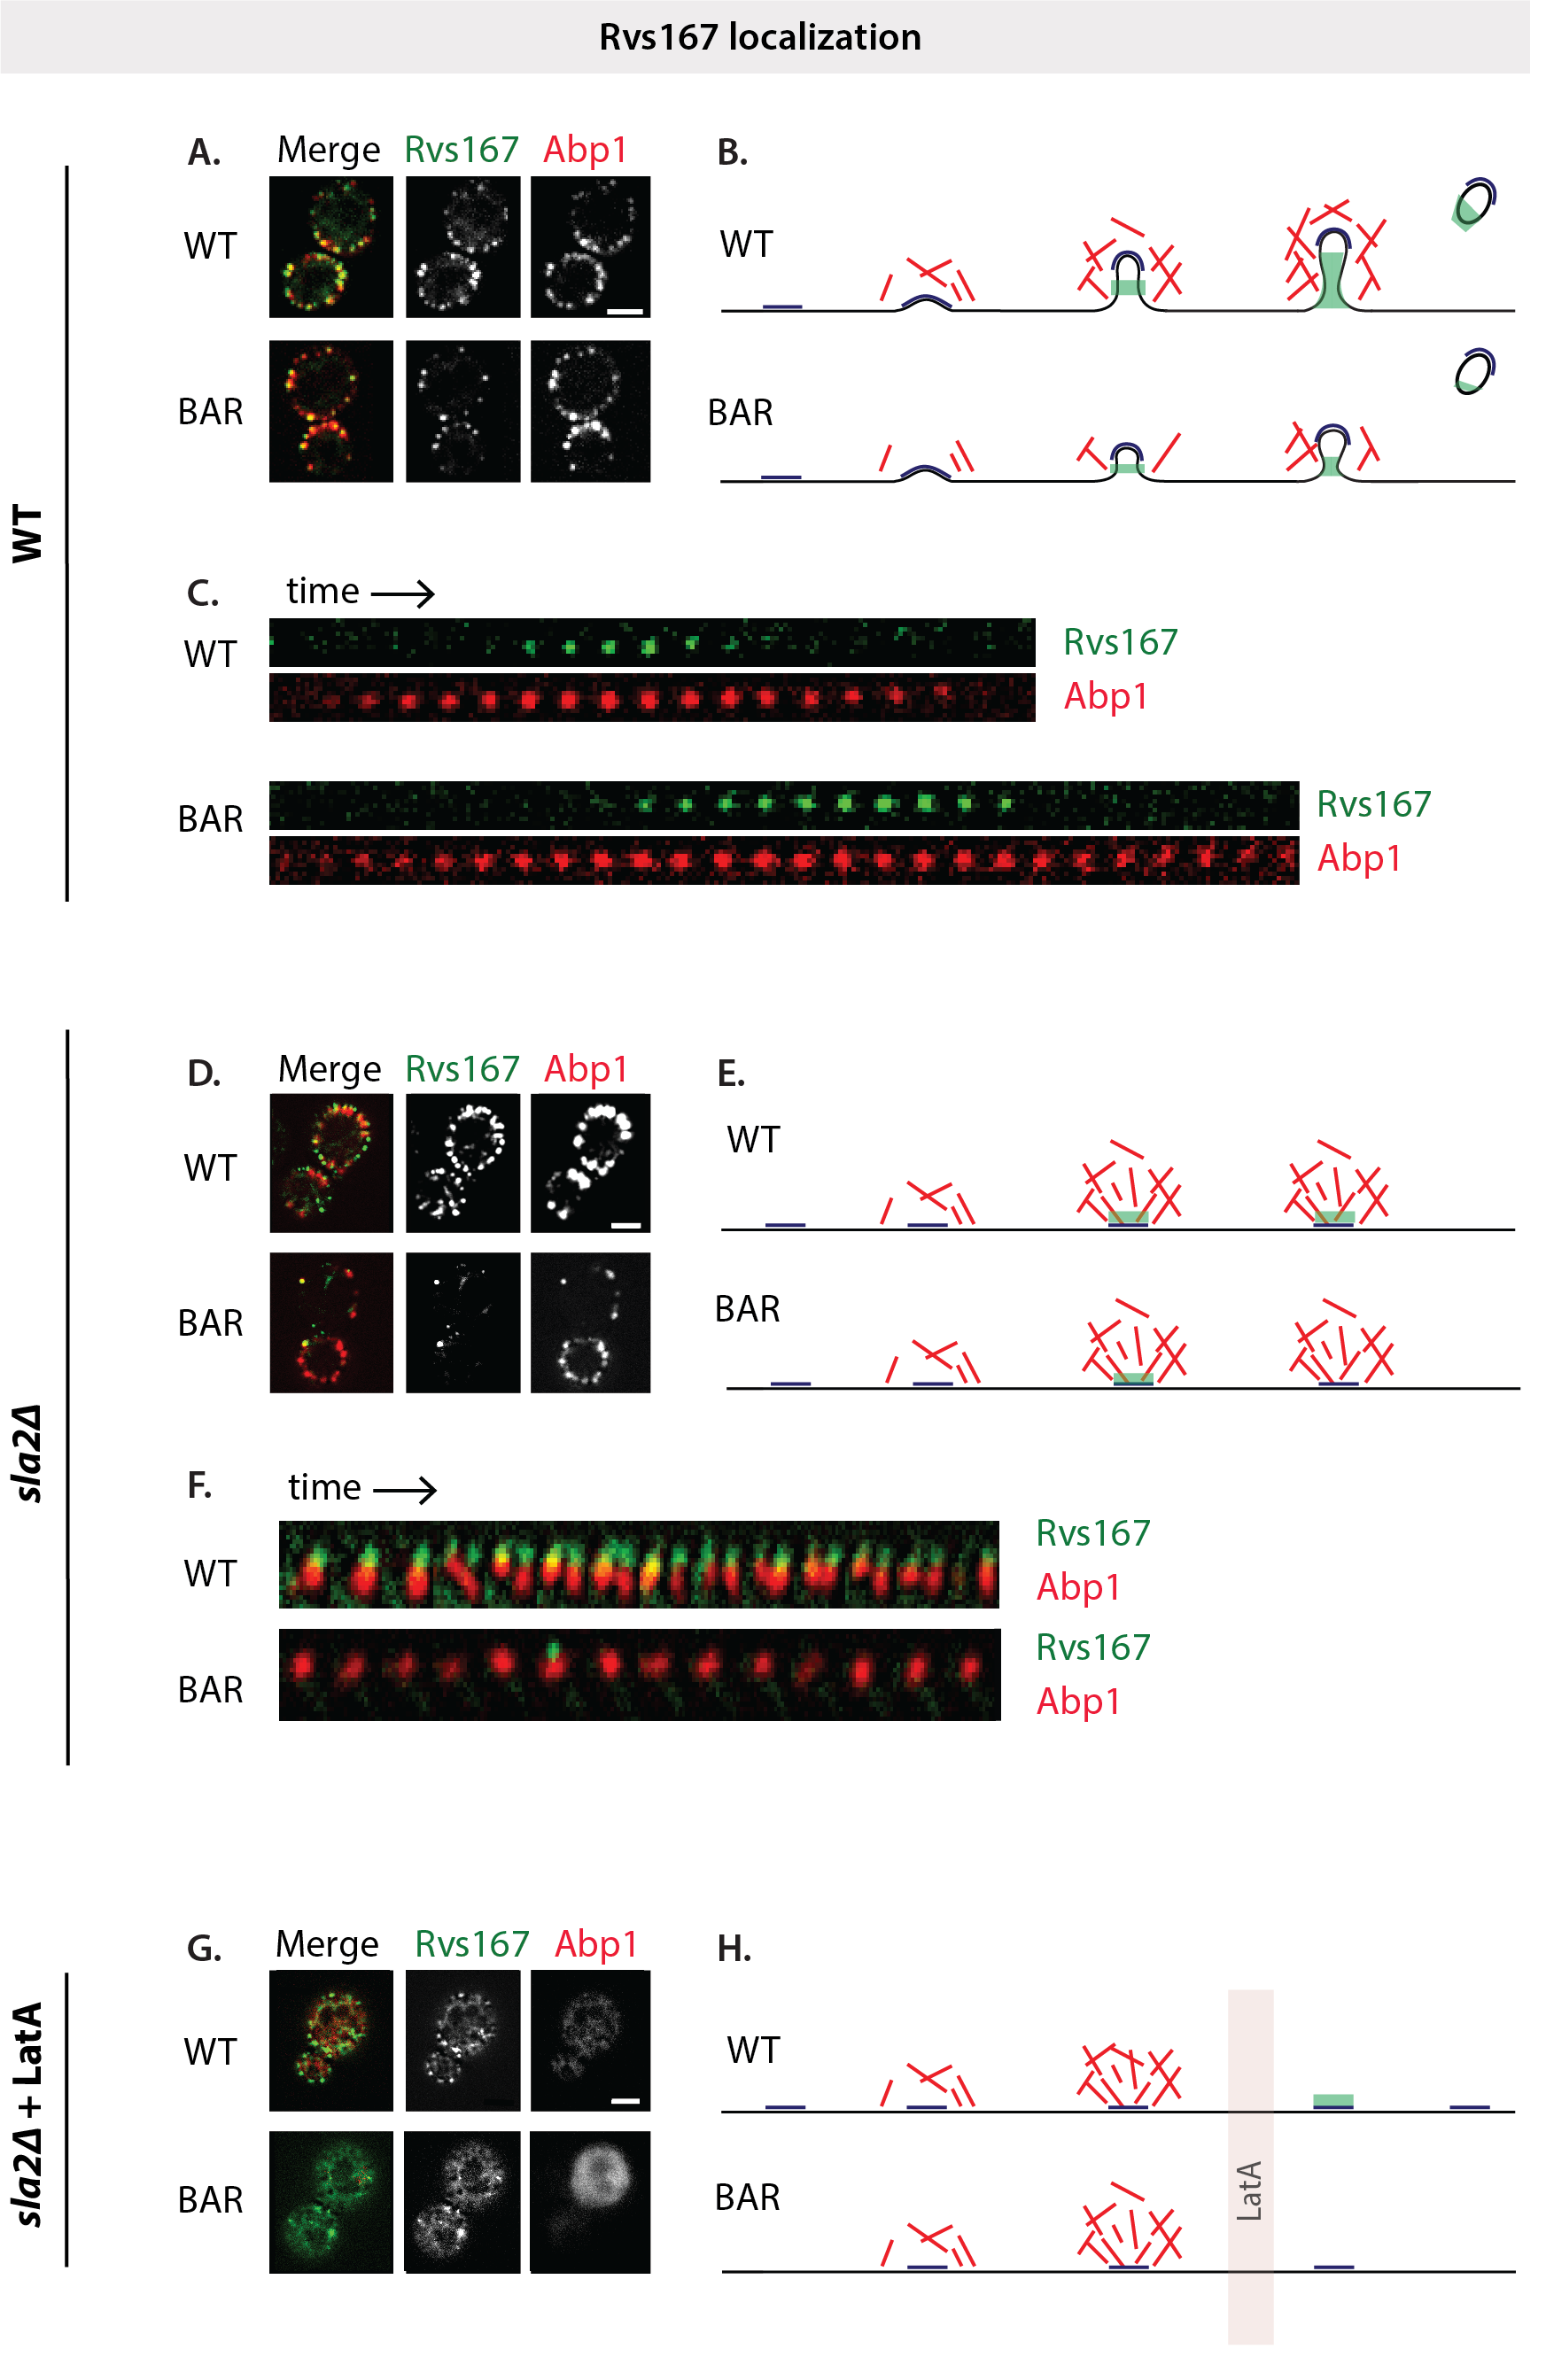
\includegraphics[width=22cm,height=22cm,keepaspectratio]{figures/results_final/sla2_del_final6}
	\caption [Localization of Rvs167 and BAR with and without membrane curvature]
	{A: Maximum intensity projections of time lapse images of Rvs167-GFP and BAR-GFP co-expressed with Abp1-mCherry. Exposure rate, 250ms for GFP and RFP channels, excited using 488 and 561nm lasers respectively. B: Schematic of membrane progression of in WT endocytic events. C: Kymograph of Rvs167-GFP and BAR-GFP localizations on the plasma membrane with Abp1-mCherry. Each frame of kymograph is every third frame from time lapse images. 
D: Maximum intensity projection of time lapse images of sla2del cells expressing Rvs167-GFP and BAR-GFP with Abp1-mCherry. E: Schematic of membrane invagination in the absence of Sla2. F: Kymograph of Rvs167-GFP BAR-GFP with Abp1-mCherry. Exposure rate 1000ms for GFP, 800ms for RFP, excited using 488 and 561nm lasers. 
G: Maximum intensity projection of time lapse images of sla2del cells expressing Rvs167-GFP and BAR-GFP, along with Abp1-mCherry, treated with LatA for 10’. Exposure rate 1000ms for GFP, 800ms for RFP. H: Schematic of membrane invagination in Sla2del cells treated with LatA. All scale bars, 2um\label{fig2_sla2del}}
\end{figure}

	\vspace{5mm}
In sla2del cells, Rvs167-GFP is recruited to the plasma membrane (Fig.2.2D,F) at the plasma membrane, and together with Abp1-mCherry. Some Rvs167-GFP patches persist at the plasma membrane, while many are assembled and disassembled at Abp1 patches. Some Rvs167 patches do not co-localize with Abp1. In sla2del cells expressing BAR-GFP, localization is mostly removed except for rare transient patches at the plasma membrane that are co-localized with Abp1, while most of the patches appear to be recruited independent of Abp1. Rvs167-GFP and BAR-GFP patches are both dynamic, indicating an interaction exists in both cases that is able to assemble and disassemble Rvs patches at the plasma membrane. 

	\subsection{The SH3 domain is able to localize Rvs in an 
		actin and \\ curvature-independent manner}

	As I show in the previous section, full-length Rvs is able to localize to cortical patches in Sla2del cells. This localization must come from the SH3 domain, since BAR alone does not localize in cells without sla2. We expected that the SH3 domain must interact with WASP or actin-binding proteins: an interaction with Abp1 has been shown, as well as with Las17, type I Myosins, and Vrp1. In order to prove this, I imaged BAR-GFP and Abp1-mCherry in sla2del cells treated with the actin sequestering agent LatrunculinA (LatA). LatA is a sea-sponge toxin that binds monomeric actin and prevents incorporation of actin into filaments. Since high actin turnover is required at endocytic sites, LatA effectively disassembles WASP components and other actin-binding proteins of the endocytic machinery, and blocks endocytosis. In combination with the sla2 deletion, latA treatment will effectively prevent membrane curvature as well as remove actin-binding proteins from endocytic sites. Loss of actin binding proteins is verified by the loss of Abp1 signal in the RFP channel.


	\vspace{5mm}
Surprisingly, full-length Rvs is transiently localized to the plasma membrane in spite of the LatA treatment, suggesting that the SH3 domain is able to recruit Rvs to the plasma membrane. This recruitment occurs in the absence of a BAR-membrane interaction, since BAR-GFP localization is completely removed in LatA treated cells. Rvs167-GFP patches are transient, so an assembly-disassembly mechanism is mediated by the SH3 domain outside of its BAR domain interaction. Localization of Rvs161, which does not have an SH3 domain, is also removed by LatA treatment12, supporting the conclusion that the BAR domains of the Rvs complex senses membrane curvature in-vivo. 

	\subsection{Loss of the SH3 domain affects endocytic progression}s
Since the SH3 domain plays a surprisingly larger role in the function of Rvs, I investigated its effect further. The SH3 domain generally mediates protein-protein interaction by binding to proline-rich sequences that contain a core PXXP motif13,14 (where X is any amino acid). These domains are ubiquitous in cellular interaction pathways, and several endocytic proteins have at least one SH3 domains, used to self-regulate activity, as well as to modulate local concentrations of protein. Although SH3 domains are abundant, they appear to have specific of binding partners. For Rvs167 SH3, neither the specific binding partner, nor its function in the scheme of endocytosis is known. From early work, the BAR domain is expected to act as the functional module of the Rvs proteins: most of the phenotypes of Rvs deletion can be compensated by expression of the BAR domain alone, although the SH3 domain is required in addition to the BAR domain for bipolar budding pattern15. 

	\vspace{5mm}
In order to probe the contribution of the Rvs SH3 domain to endocytosis, I studied coat and Rvs dynamics by expressing Rvs167 without the SH3 domain. Quantification of the number of BAR-GFP molecules reruited to endocytic sites shows that without the SH3 domain, recruitment is reduced by half (30.1 +/- 9.9 for BAR-GFP compared to 53.2 +/- 5.3 for Rvs167-GFP), although the cytoplasmic concentration of protein is not affected compared to Rvs167-GFP. The inward jump of BAR-GFP is reduced, compared to the full-length protein, and a number of BAR-GFP patches remain on the plasma membrane and are disassembled without inward movement. Movement of the coat protein Sla1 is similarly reduced. Sla1 moves in to approximately 50nm instead of the 140nm found in WT invaginations. Abp1-GFP recruitment without the SH3 domain is reduced to 50\% of WT recruitment, from 347+/- 30.6 molecules in WT to 172.6 +/- 12.9. Shorter invaginations with a maximum of 60nm have been observed in the case of Rvs167 deletion by CLEM 10, which is about the same length as those observed in the SH3 deletion: loss of the SH3 domain appears to be detrimental to the function of the Rvs complex.

\begin{figure}
	\centering
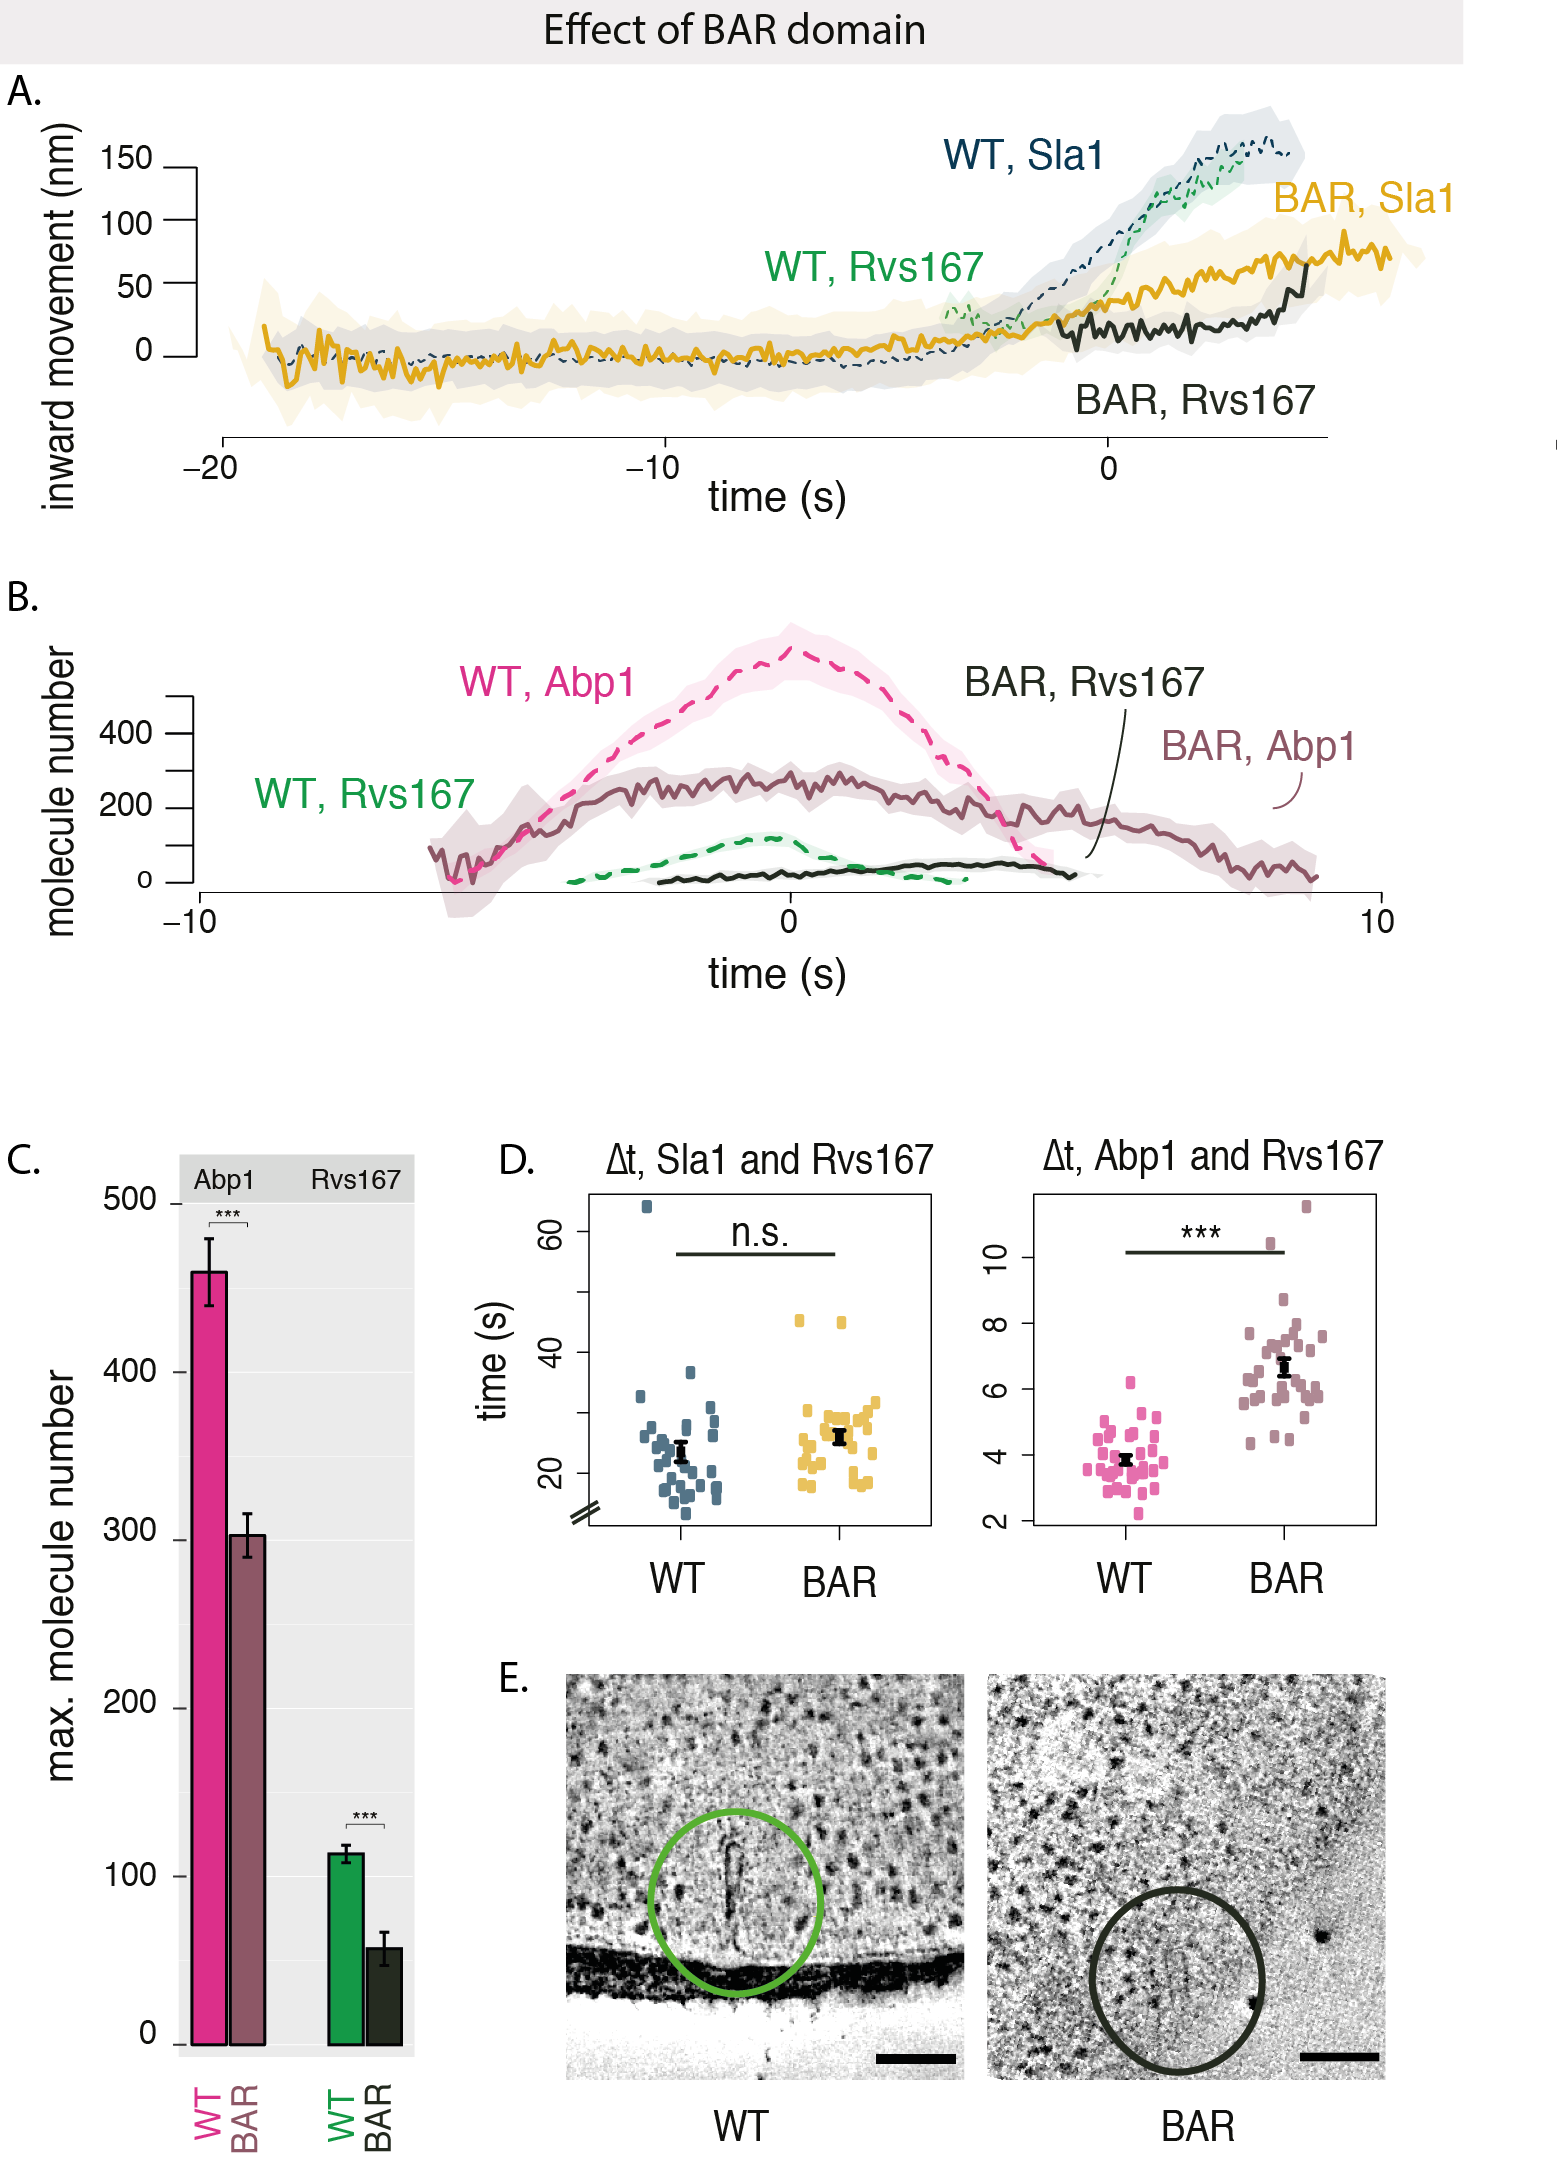
\includegraphics[width=19cm,height=19cm,keepaspectratio]{figures/results_final/delsh3_6}
	\caption [Effect of the Rvs167 SH3 deletion]
	{A: Averaged centroid movement of Sla1 and Rvs167 in WT and BAR strains. Centroids are aligned in time so that time=0 corresponds to the Abp1-mCherry fluorescent intensity peak in simultaneous dual-color imaging of the corresponding strains. Exposure rate 250ms.
B: Molecule numbers of Abp1-GFP and Rvs167-GFP and BAR-GFP with standard error of mean. 
C: Lifetimes are measured by TIRF in Rvs167-GFP/ Abp1-mCherry and Rvs167-GFP/ Sla1-mCherry strains in WT and BAR strains. Exposure 560ms for each channel. Mean and standard error of the mean are shown,  * = p $\leq$ 0.05 , ** = p$\leq$ 0.01, *** = p $\leq$ 0.001 . P values of two-sided t test. 
D: Difference in time between arrival of Sla1-mCherry and Rvs167-GFP, and Abp1-mCherry and Rvs167-GFP in WT and BAR strains. Exposure 560ms for each channel. Mean and standard error of the mean are shown, * = p$\leq$ 0.05, ** = p$\leq$ 0.01, *** = p$\leq$ 0.001. P values of two-sided t test.\label{fig2_sh3del}}
\end{figure}
	\vspace{5mm}
	
For a more detailed inquiry into changes in the endocytic machinery without the Rvs167 SH3 domain, I quantified the lifetimes of Rvs, and coat and actin network using Sla1 and Abp1 as markers in SH3 deleted cells using total internal reflection fluorescence (TIRF) microscopy. Unlike epifluorescence microscopy at the equatorial plane, that has been the method used for quantification so far, when using TIRF, only fluorophores up to a depth of about 100nm from the glass-sample interphase are excited. This reduces fluorescent signal from the cytoplasm, allowing detection of low intensity fluorescent signal, and is a better method for quantification of protein lifetime than epifluorescence microscopy. Lifetimes of BAR-GFP, Sla1-mCherry and Abp1-mCherry in SH3 deleted cells is compared against WT Rvs167-GFP, Sla1-mCherry and Abp1-mCherry. 

\begin{figure}
	\centering
	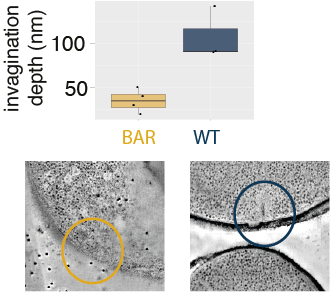
\includegraphics[width=5cm,height=5cm,keepaspectratio]{figures/results_final/clem}
	\caption [Effect of the Rvs167 SH3 deletion]
	{Length of invaginations from correlative light and electron microscopy for WT and BAR strains}
\end{figure}
\vspace{5mm}
	
	\vspace{5mm}
While the lifetimes of Rvs167 and BAR are similar, and Sla1 lifetime with and without the SH3 domain is also similar, there is a significant increase in the lifetime of Abp1 lifetime in the absence of the SH3 domain. I then looked for differences in the sequence of recruitment of these endocytic proteins by looking at the difference in time between recruitment of Sla1 and Rvs, and the difference in time between recruitment of Abp1 and Rvs in the WT and SH3 deleted strain. The time difference between recruitment of Sla1 and full-length and SH3 deleted Rvs167 is unchanged, while the difference in time between recruitment of Abp1 and BAR is increased when compared to WT Rvs.

	\subsection{What does the SH3 domain interact with?}
		\subsubsection{Vrp1}
		\subsubsection{Type 1 myosins}
		\subsubsection{Las17}


	\subsection{Other potential mechanisms of assembly/ disassembly of Rvs}		
			\subsubsection{Interaction with Calmodulin}
			\subsubsection{FBAR protein Bzz1}
				
\section{Role of the SH3 domain}	
Is likely that SH3 domains, are involved in modulating oligomerization (5, 14) and MC-S, G (15, 82). 	
\section{Role of the N-helix}			
		
\section{Scission mechanisms}

	\subsection{Membrane scission is not dependent on Vps1}
	Yeast dynamin is the obvious solution to membrane scission. Although none of the three dynamin- like proteins has a proline-rich domain, one of the yeast dynamins, Vps1 has been suggested to be involved in endocytosis11,12. Rooij et al., suggest that Vps1 localizes to endocytic sites in the late scission stage, and that the vps1Δ rvs167Δ double mutant increases membrane retraction rates after invagination, an indication of scission failure. Vps1-GFP does not localize to endocytic sites in Gadila et at.,13, but localizes to the golgi body and to vacuoles. Kishimoto et al, do not find a colocalization between Vps1 and Abp1 localization, and also report that the vps1Δ rvs167Δ  double mutation does not affect membrane retraction rates. Vps1 tagged with both GFP as well as superfolded GFP, and imaged by TIRF microscopy fails to colocalize with Abp1 (data not shown, personal communication with Andrea Picco). The debate concerning the involvement of Vps1 in membrane scission in yeast has been compounded by the possibility that the GFP tag at the Vps1 C-terminal could interfere with its localization to endocytic sites, or its interaction with the Rvs complex. 
	
	\vspace{5mm}
	In order to exclude the possibility of interference from the GFP tag, I investigated the role of Vps1 by studying coat and scission proteins in vps1Δ cells. The late coat protein, Sla1 is used as a marker for coat movement, and Rvs167 marks scission time. Centroid tracking and averaging is performed as described in Picco et al., and inward movements of the both in wild-type and vps1Δ cells are compared. 

%	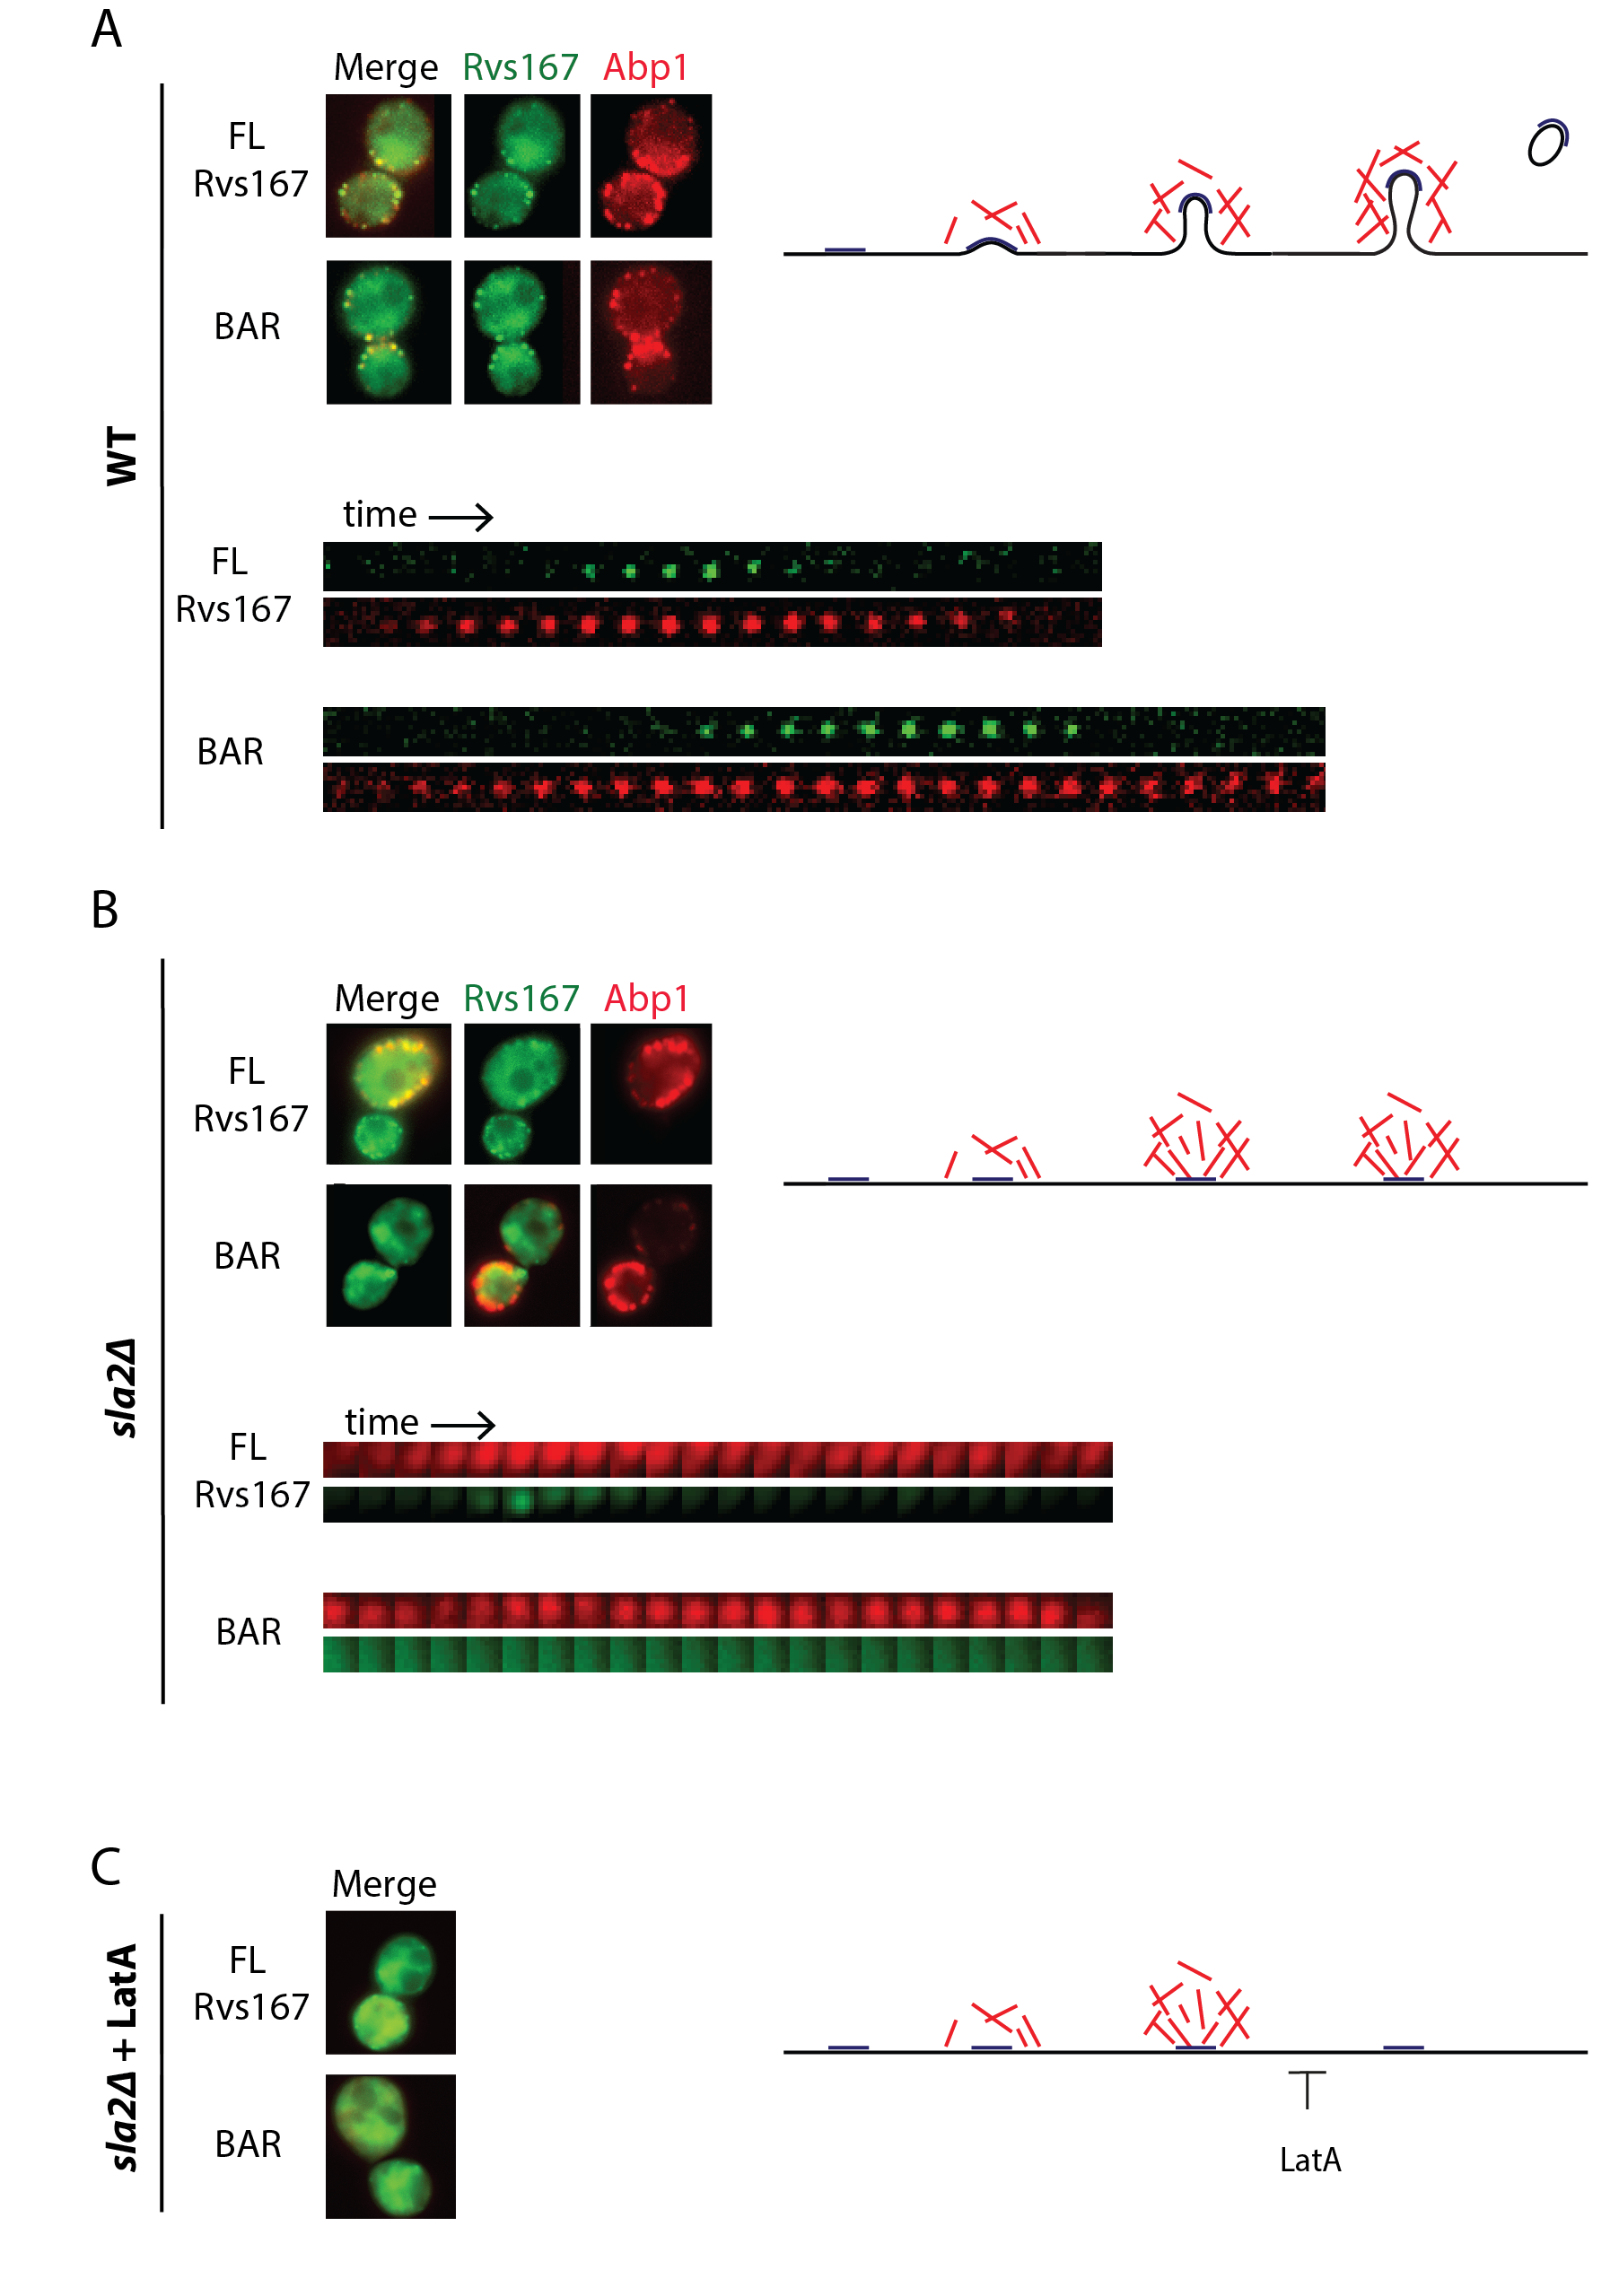
\includegraphics[width=20cm,height=20cm,keepaspectratio]{../../../figures/results_final/sla2_del_final3}
	\begin{figure}
	\centering
	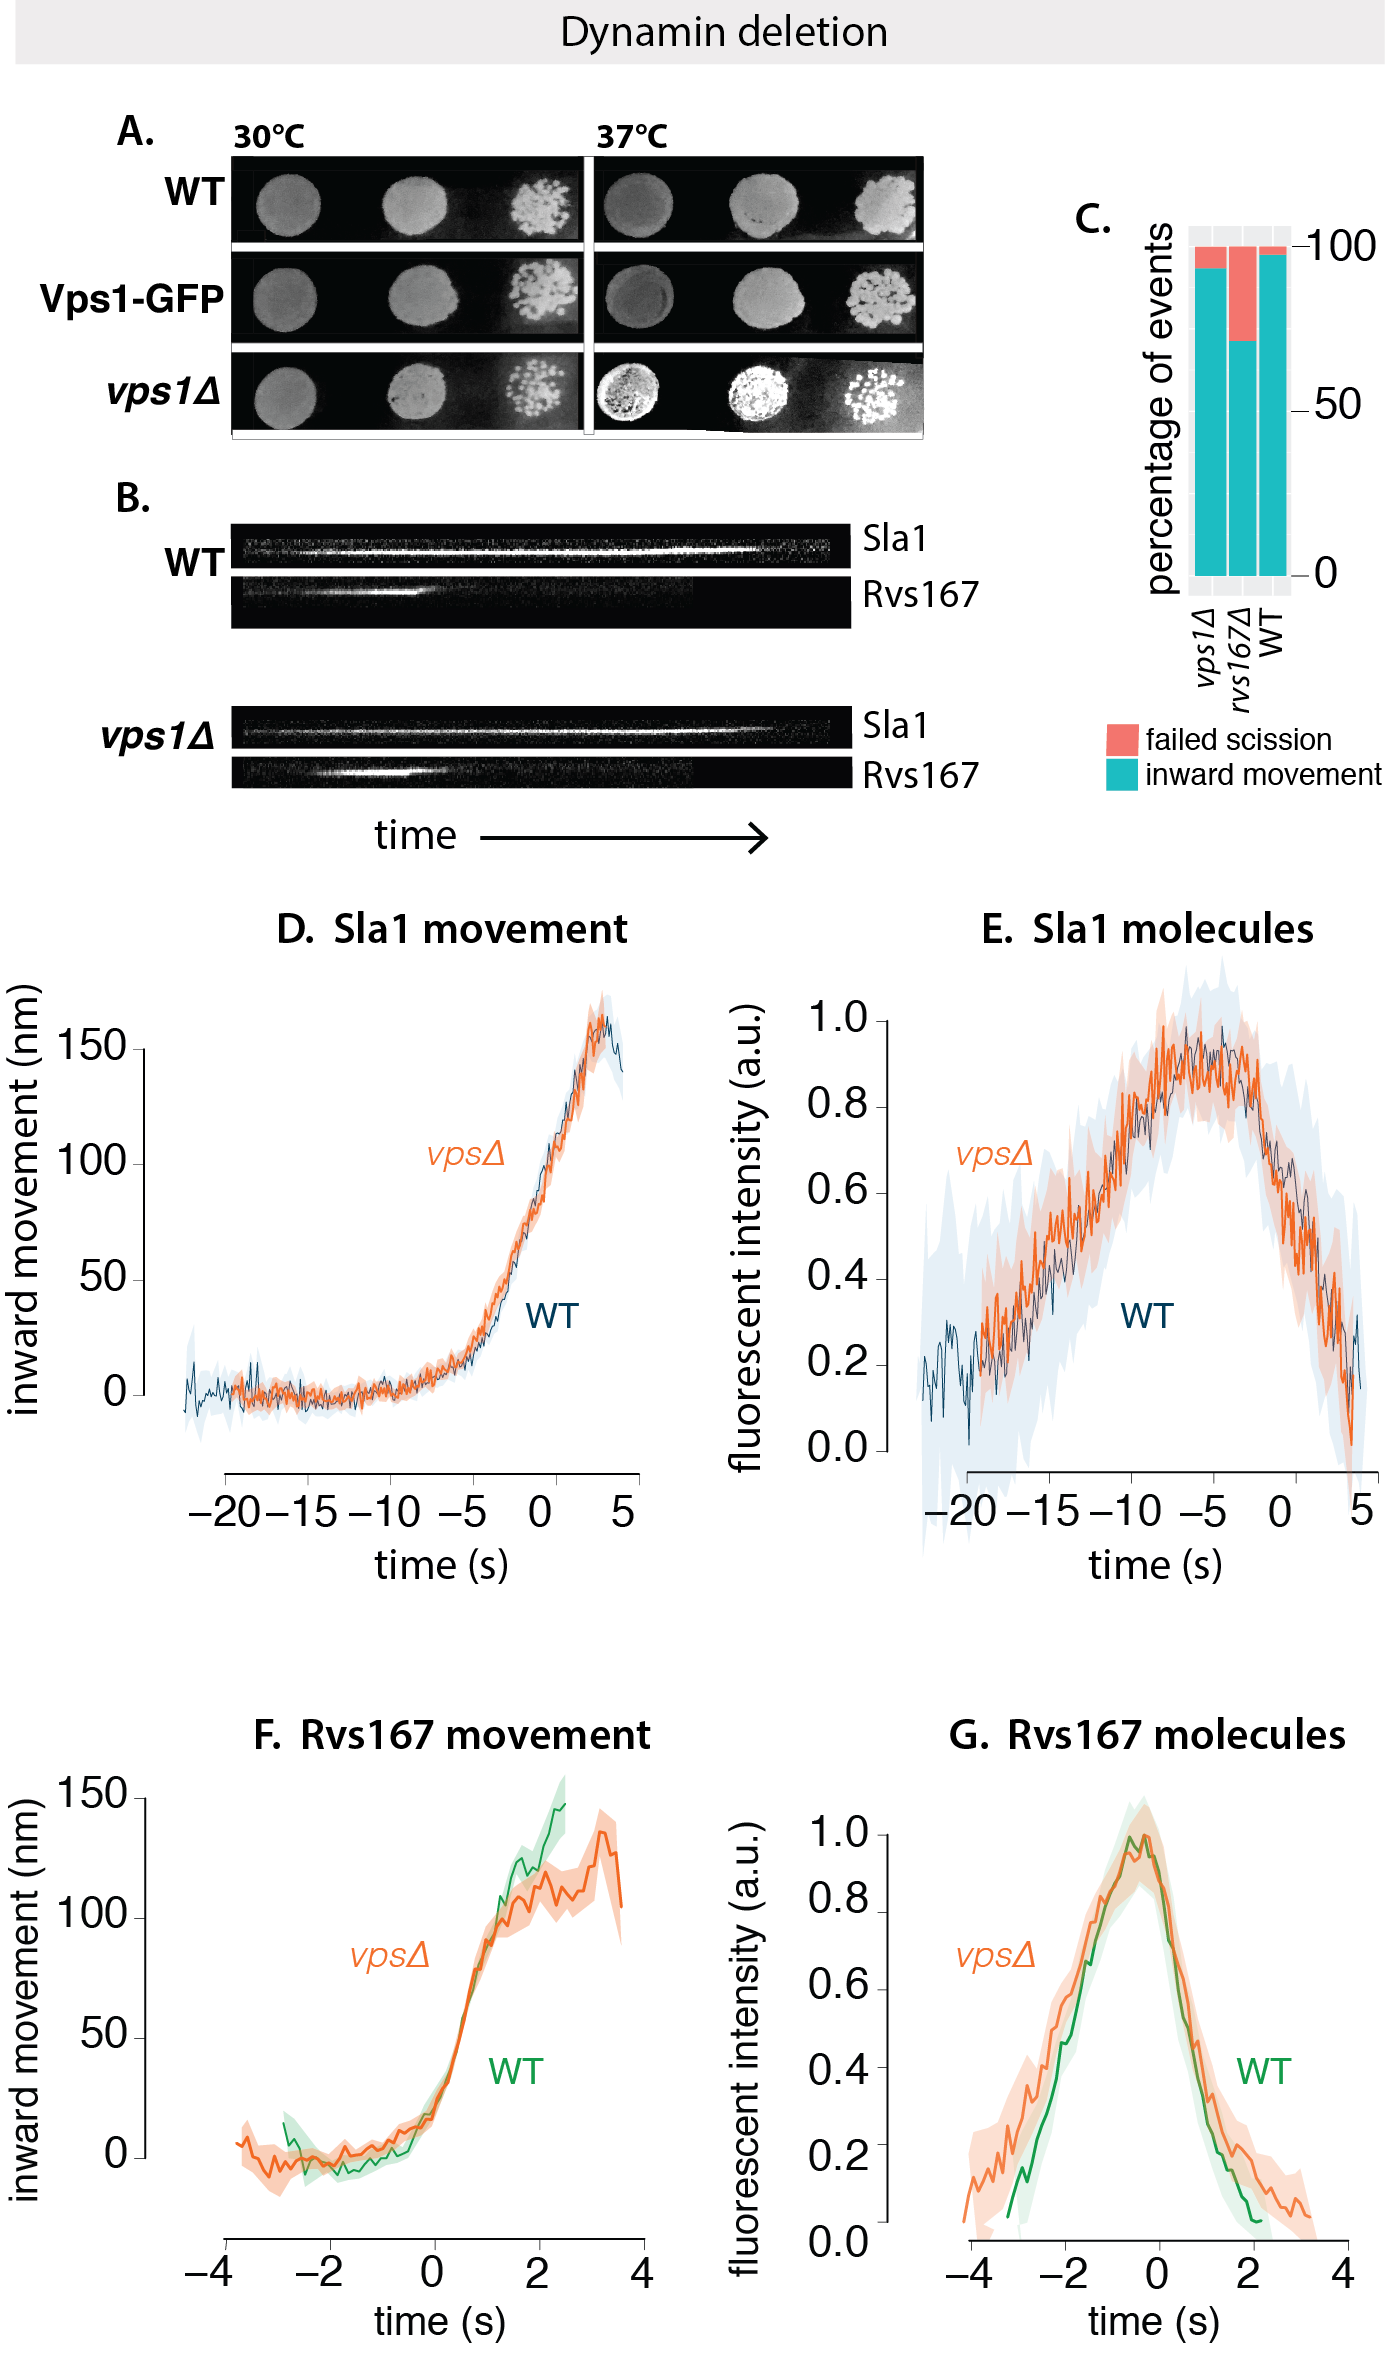
\includegraphics[width=20cm,height=20cm,keepaspectratio]{figures/results_final/vps}
		\caption{Rvs localization in vps deletion\label{fig3_vpsdel}}
	\end{figure}

	
	\vspace{5mm}
	vps1Δ cells exhibit a growth defect at 37C, as has been reported11. Sla1-GFP accumulates at the plasma membrane, moves inwards, and disassembles like in WT. The average lifetime of Sla1-GFP at endocytic patches remains unchanged. In WT cells, Sla1 moves into the cytoplasm about 140nm before membrane scission occurs. If Vps1 was required for membrane scission, Sla1 would be expected to undergo delayed or failed scission. However, vps1Δ does not increase the rate of membrane retraction. Inward movement of Sla1 is also not changed: it moves inward at the same rate, and to similar maxima of 140nm. Further, the averaged centroid of Rvs167 would not show the sharp jump into the cytoplasm if scission failed. If scission was delayed, the average lifetime of Rvs167 would increase. The inward movement of Rvs167, and its average lifetime, however, remains the same as in WT. I conclude that if Vps1 does localize to endocytic patches in S.cerevisiae, it is not involved in regulating membrane scission.  


	\subsection{Lipid hydrolysis and membrane scission}
	
	\subparagraph{Can lipid hydrolysis drive membrane scission?}
	Another hypothesis has proposed that regulated lipid hydrolysis can cause vesicle scission19. Phosphatidylinositols (PIs) and their derivatives play important roles in many cellular processes including membrane trafficking and cell signalling. Conversion between lipid types is driven by kinases, lipases, and phosphatases and controlled throughout the membrane trafficking pathway. 
	
	\vspace{5mm}
	Phosphatidylinositol(4,5)-biphosphate (PI (4,5) P2) is an important lipid type found at the cell surface, and is enriched and depleted from endocytic sites at the plasma membrane in concert with the assembly and disassembly of the endocytic machinery. Synaptojanins form a subset of inositol polyphosphate 5-phosphatases that hydrolyze PI(4,5)P2 to PI(4)P by removing the phosphate at the 5’ position of the inositol ring, and play a role in CME and intracellular signalling, as well as in modulating the actin cytoskeleton14. Synaptojanins localize to endocytic sites, and in mammalian cells, disruption of Synaptojanin genes results in cellular accumulation of PI(4,5)P2 and coated vesicles at the plasma membrane, suggesting a role for lipid hydrolysis in releasing coat proteins from nascent vesicles. Syaptojanins contain an N-terminal homology domain with the cytoplasmic domain of the yeast SAC1 gene, that is implicated in lipid metabolism, actin morphology, and vesicle transport in the secretary pathway15. A central catalytic domain is followed by a proline-rich C-terminal regions that are the canonical interaction partners of SH3 domains: they are known to interact with actin binding proteins and BAR domain proteins, potentiating also a role in membrane invagination and scission. 
		
	\vspace{5mm}
	The yeast encodes three Synaptojanin-like proteins- Inp51, Inp52 and Inp53- that regulate phospholipid metabolism. Double deletion of Inp51 and Inp52 has been shown to increase the lifetime of endocytic proteins and produce aberrant membrane invaginations that could indicate scission failure and defective endocytosis, although uptake of extracellular membrane appears to proceed in spite of the morphological aberrations16,17. Deletion of Inp52 along with Rvs167 increases scission failure rate, supporting a possible role in membrane scission18. Loss of inp51 mutation shows a increase in bulk PIP2 level, although chages in PIP2 levels have not been reported for mutations of inp52, and are not measured locally at the endocytic sites19,20.

	\subparagraph{Loss of yeast synaptojanins does not significantly affect coat and Rvs dynamics}
	\mbox{}\\
	In a model proposed by Liu et al, Synpatojanins and BAR proteins interact to regulate PI(4,5)P2 hydrolysis, which in turn drives membrane scission. Here, the Rvs scaffold on the membrane tube protects the underlying PIP2 from hydrolysis. Synaptojanin arrives at sites, and hydrolyses unprotected PIP2. This generates a boundary between BAR-protected PIP2 at the tube and PIP at the bud tip. The lipid boundary produces a line tension at the interphase that would generate enough force to pinch off a vesicle. 
	
		\begin{figure}
		\centering
		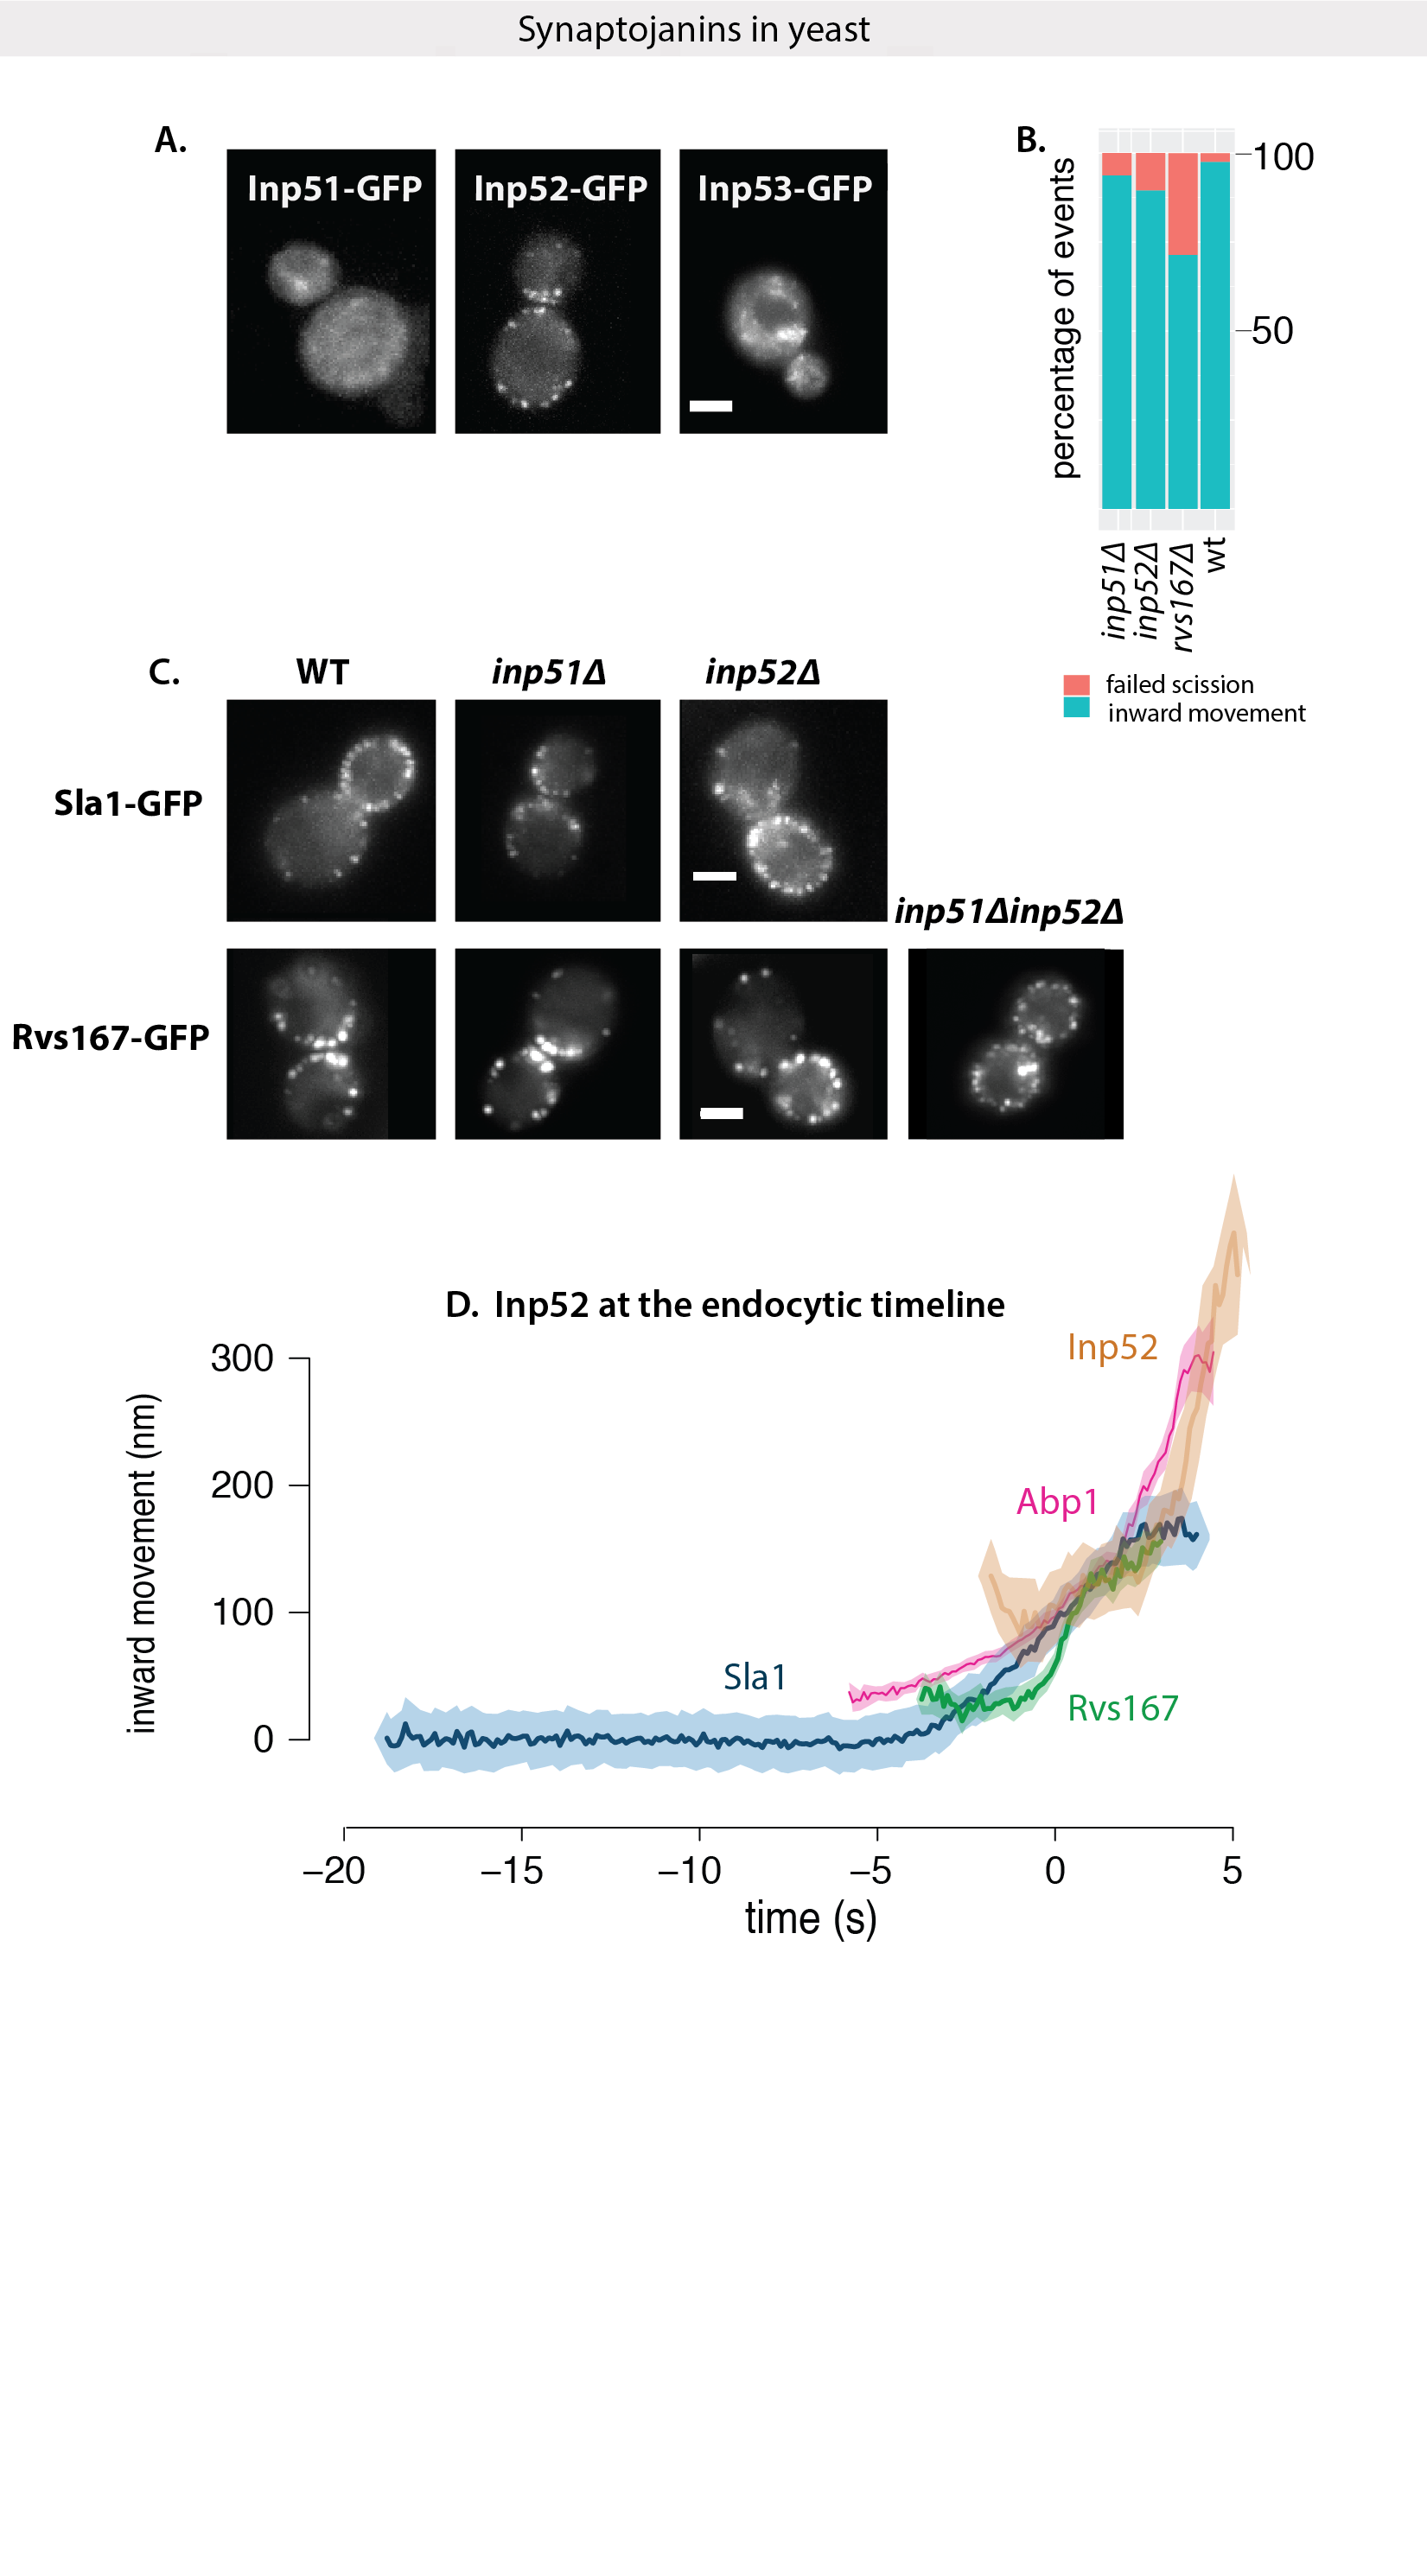
\includegraphics[width=22cm,height=22cm,keepaspectratio]{figures/results_final/inp}
		\caption{Yeast synaptojanins \label{fig4_inp}}
		\end{figure}
		
		\begin{figure}
		\centering
		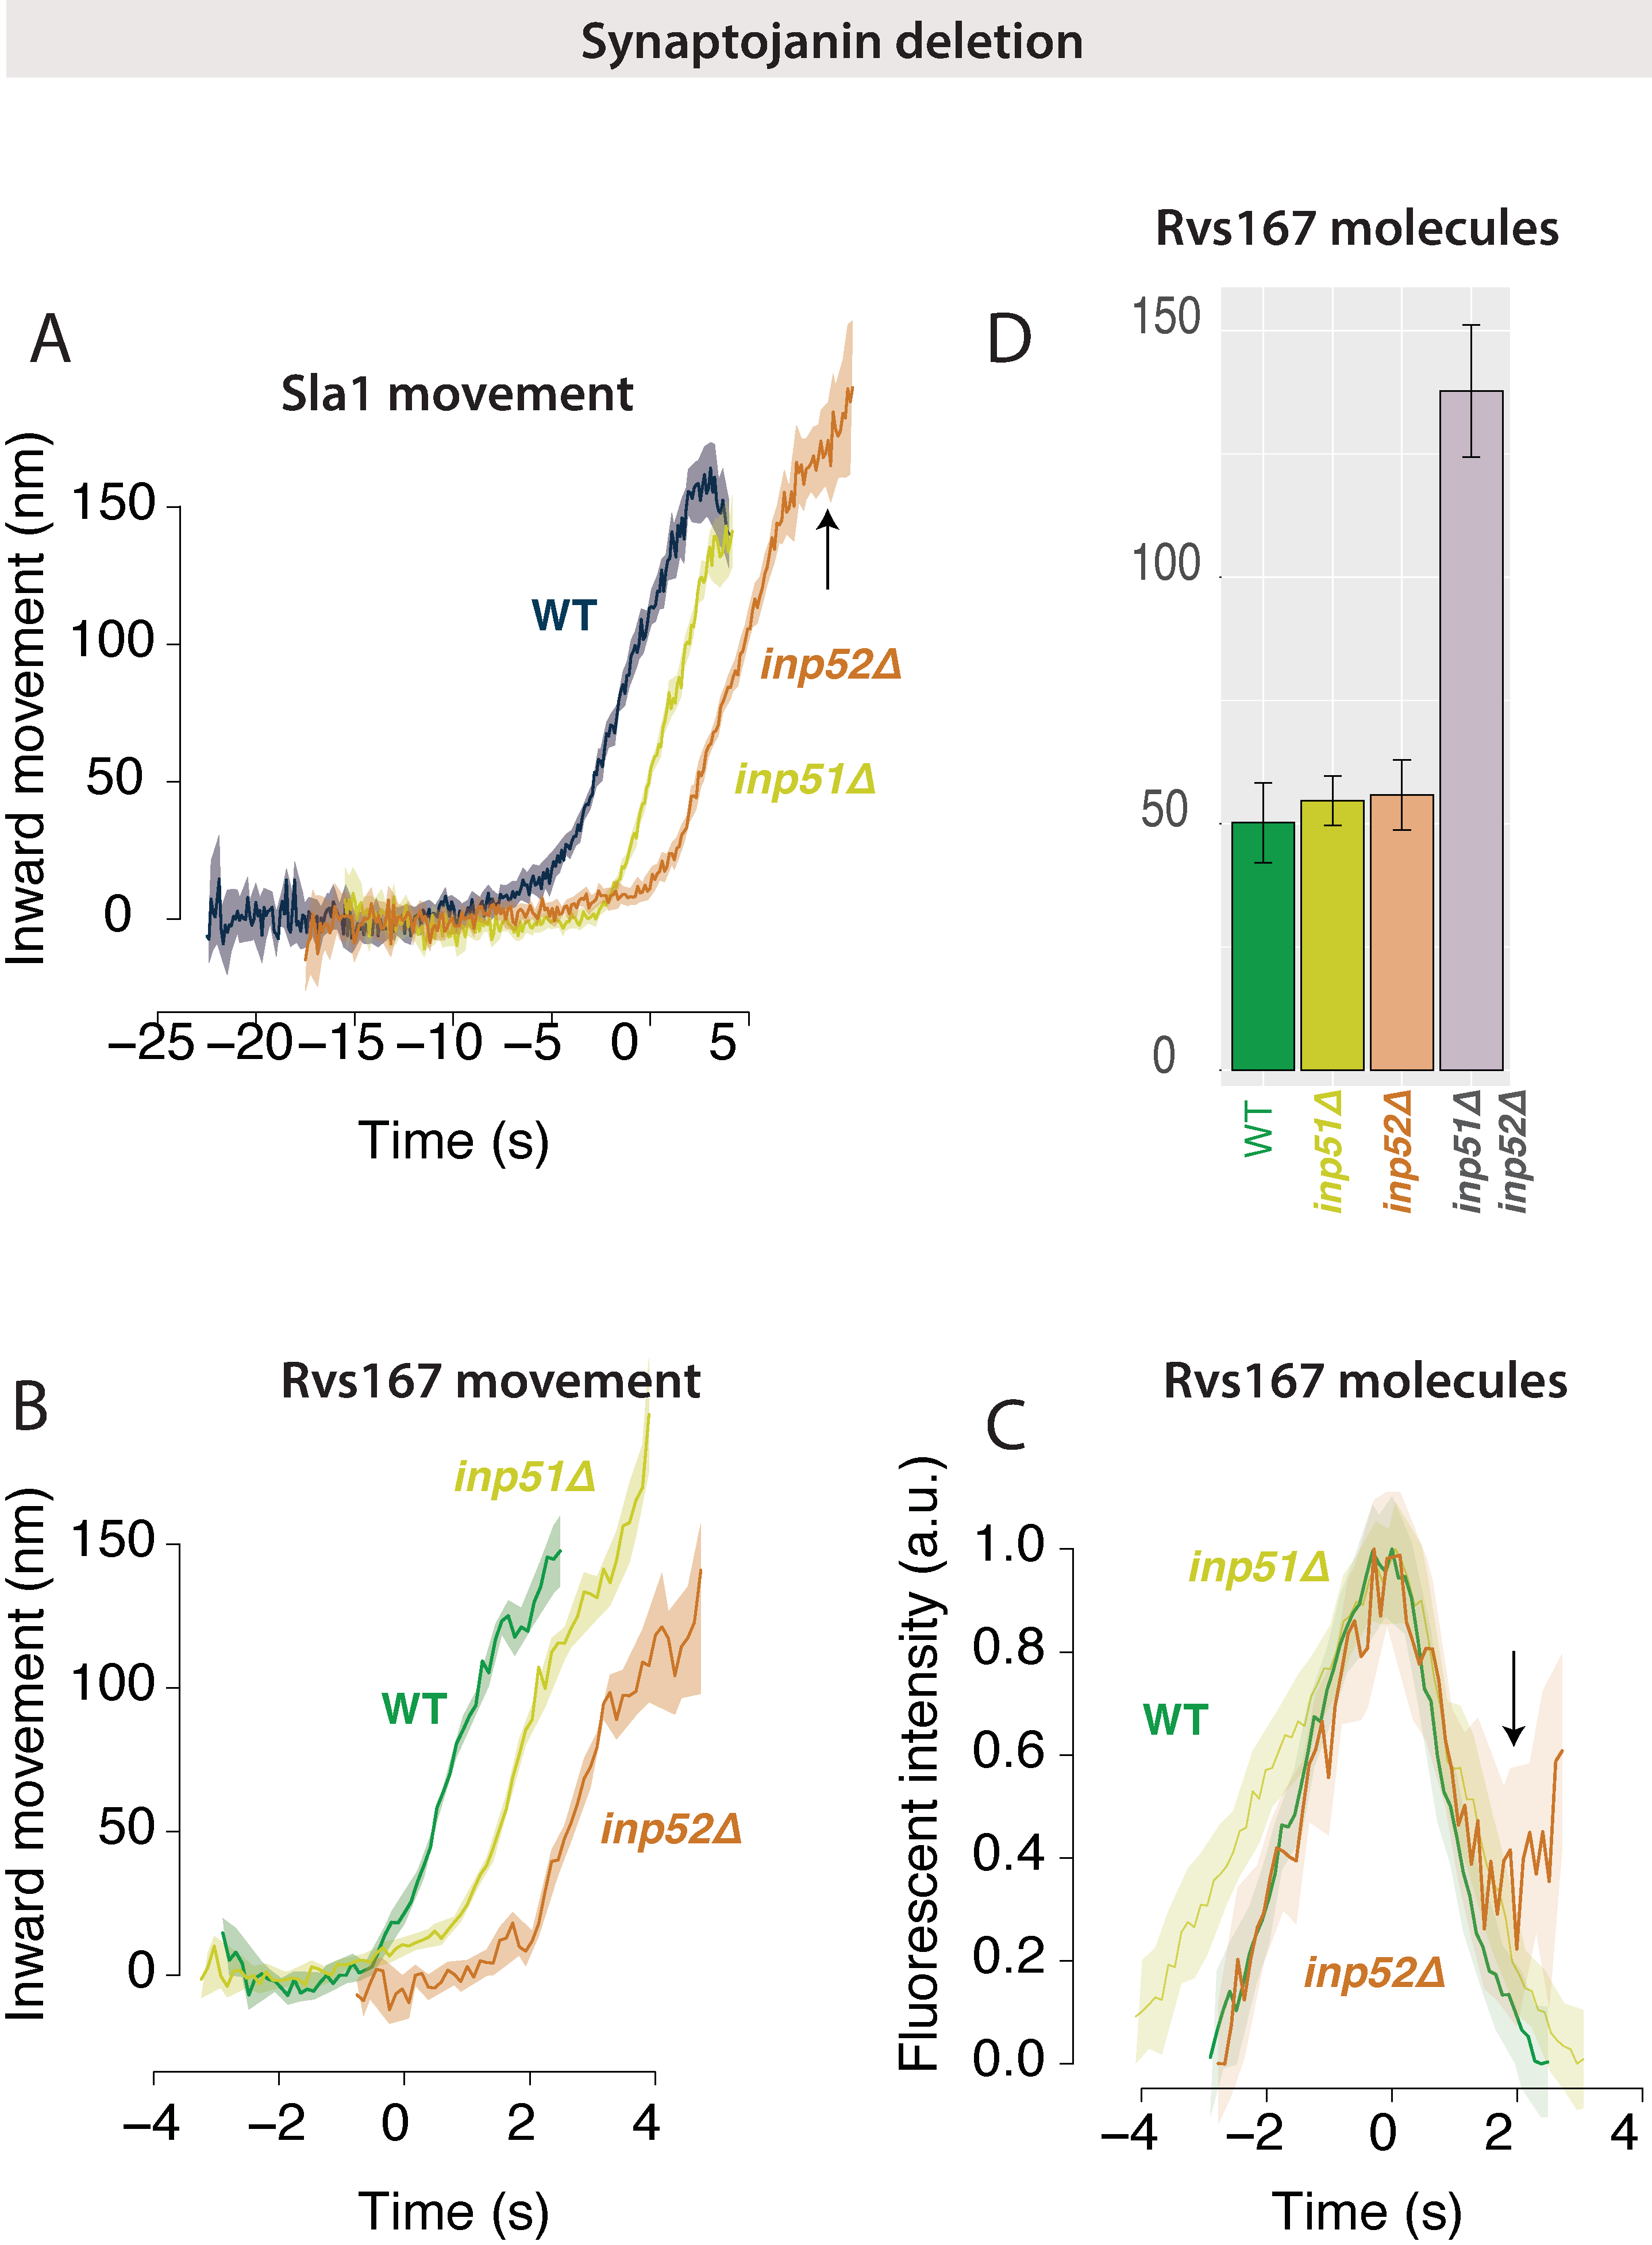
\includegraphics[width=17cm,height=17cm,keepaspectratio]{figures/results_final/inp_movement}
		\caption{Sla1 and Rvs167 in Synaptojanin deletion \label{fig5}}
		\end{figure}		

	\vspace{5mm}
	I tested this model by investigating the effect of synaptojanin deletion on coat and scission proteins. First, of the three yeast Synaptojanins, only Inp52-GFP localizes to cortical patches. Dual-color imaging and time alignment with Abp1 as described in Picco et al., shows that Inp52 localizes to endocytic sites at the late stage of scission along with Rvs. The centroid of Inp52-GFP can be localized to the tip of the invaginated tube, consistent with the Liu theory of membrane scission: spatial and temporal localization is consistent with influence on scission. Inp51-GFP exhibits a diffuse cytoplasmic signal, while Inp53 localizes to patches within the cytoplasm, likely to the trans-golgi network, as has been noted in other work. 



	\vspace{5mm}
	Deletion of Inp52 does not affect the speed of membrane invagination, as reported by the movement of the Sla1 centroid. Sla1-GFP patches are assembled and disassembled, as are Rvs167-GFP patches. All Sla1-GFP patches in the movies analysed (n=13 cells) move inwards.  Dense clusters at bud neck are not considered. 72.9\% of Rvs167-GFP patches move inwards into the cytoplasm (n=4 cells, 37patches). Remaining patches are disassembled without apparent inward movement. Dense clusters at bud neck are not included in the statistics. Vesicle scission appears to occur similar to wild-type, since the Rvs167 centroid moves inwards to approximately the same distance into the cytoplasm, indicating that the base of the vesicles are likely at the same position as in wild-type. Both Sla1 and Rvs167 centroids however, persist post-scission (arrowheads in figure) instead of disassembling immediately like in the WT. Since majority of the patches move inwards, and the increase in the lifetime of Rvs is post-scission, I find that the data is consistent with a role for Inp52 in vesicle uncoating, rather than a primary role in membrane scission, with the aberrations in plasma membrane morphology consequent of failure to recycle components, rather than scission. 
	


	\vspace{5mm}
	Deletion of Inp51 does not affect Rvs167 or Sla1 centroid movement. All Sla1-GFP patches move inward (n=19 cells). 93\% of Rvs167-GFP patches move inward (n=3 cells, 44 patches), similar to WT. Assembly of Rvs167 in the Inp51del is slowed, the implication of this delay is not thus far clear. 


	
	\subsection{Does protein friction induce membrane scission? }
	
	Recent in-vitro experiments have proposed protein friction as a mechanism by which membrane scission could occur via BAR domain proteins in the absence of dynamin24. In this model, a BAR domain scaffold on a membrane tube forms a frictional barrier to lipid diffusion. Forces that pull on the membrane, such as those exerted by motor proteins like myosins or actin polymerization, increase the frictional force exerted by the scaffold on the underlying membrane tube, increasing membrane tension in the bare region of the tube caused by membrane thinning from the lack of lipid influx to this region. Eventually, membrane pores form in this portion of the tube, leading to breaking the tube, and formation of a vesicle. Such a friction-dependent membrane scission model would predict that if more BAR proteins are added to the membrane, frictional force would increase, and scission should occur faster, that is, at shorter invagination lengths than with fewer BAR proteins. Essentially, this model requires a friction-inducing BAR scaffold, and a force that pulls the membrane under it. In yeast CME, this combination is provided by the Rvs complex and polymerization of the actin network respectively. 
	

	\subparagraph{Membrane scission does not occur at shorter tube lengths when amount of Rvs is increased}
		\mbox{}\\
		\begin{figure}
		\centering
		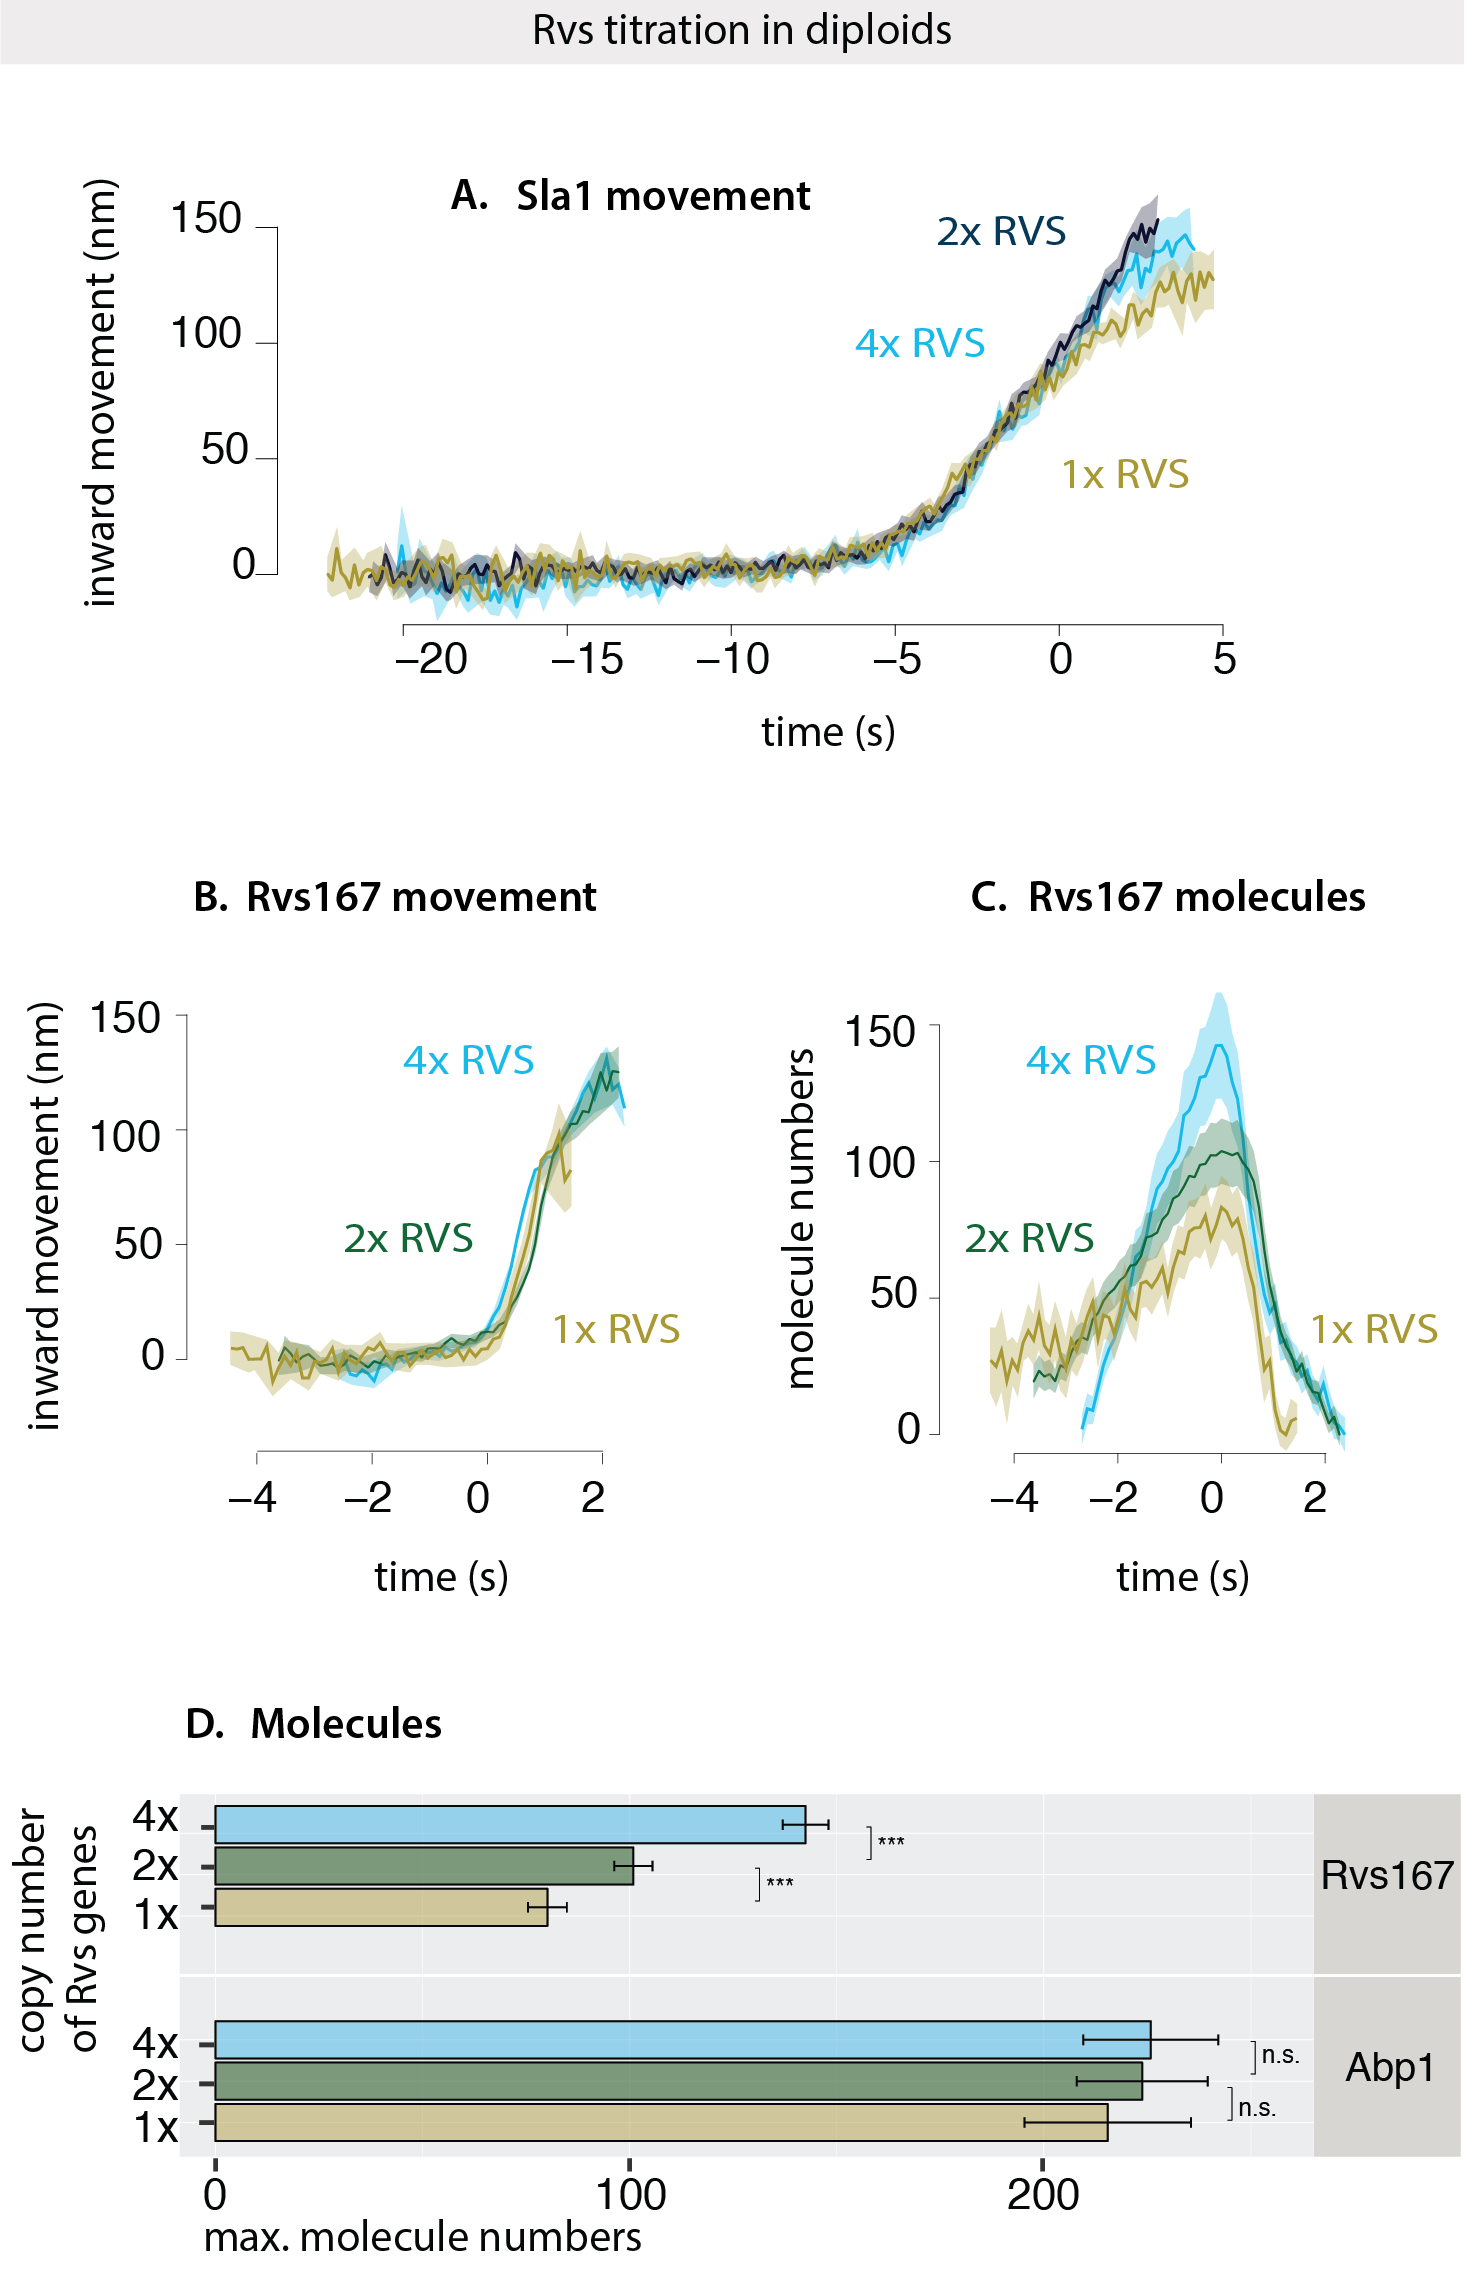
\includegraphics[width=17cm,height=17cm,keepaspectratio]{figures/results_final/protein_friction2}
		\caption{Sla1 and Rvs167 in Synaptojanin deletion \label{fig5}}
		\end{figure}
	To test whether protein friction could influence membrane scission in yeast, we duplicated the Rvs167 and Rvs161 genes as described in Huber et al.21. Gene duplication is performed in haploid cells to produce strains that have one (WT number) and two copies of both Rvs161 and Rvs167. These haploid strains are then crossed, so that diploid strains are generated that have 4x copies of the Rvs167 and Rvs161 genes, 2x copies each (WT number). Strains containing 1x copy of each Rvs is generated by crossing rvs167del strain with an rvs161del strain.
	


		\begin{figure}
		\centering
		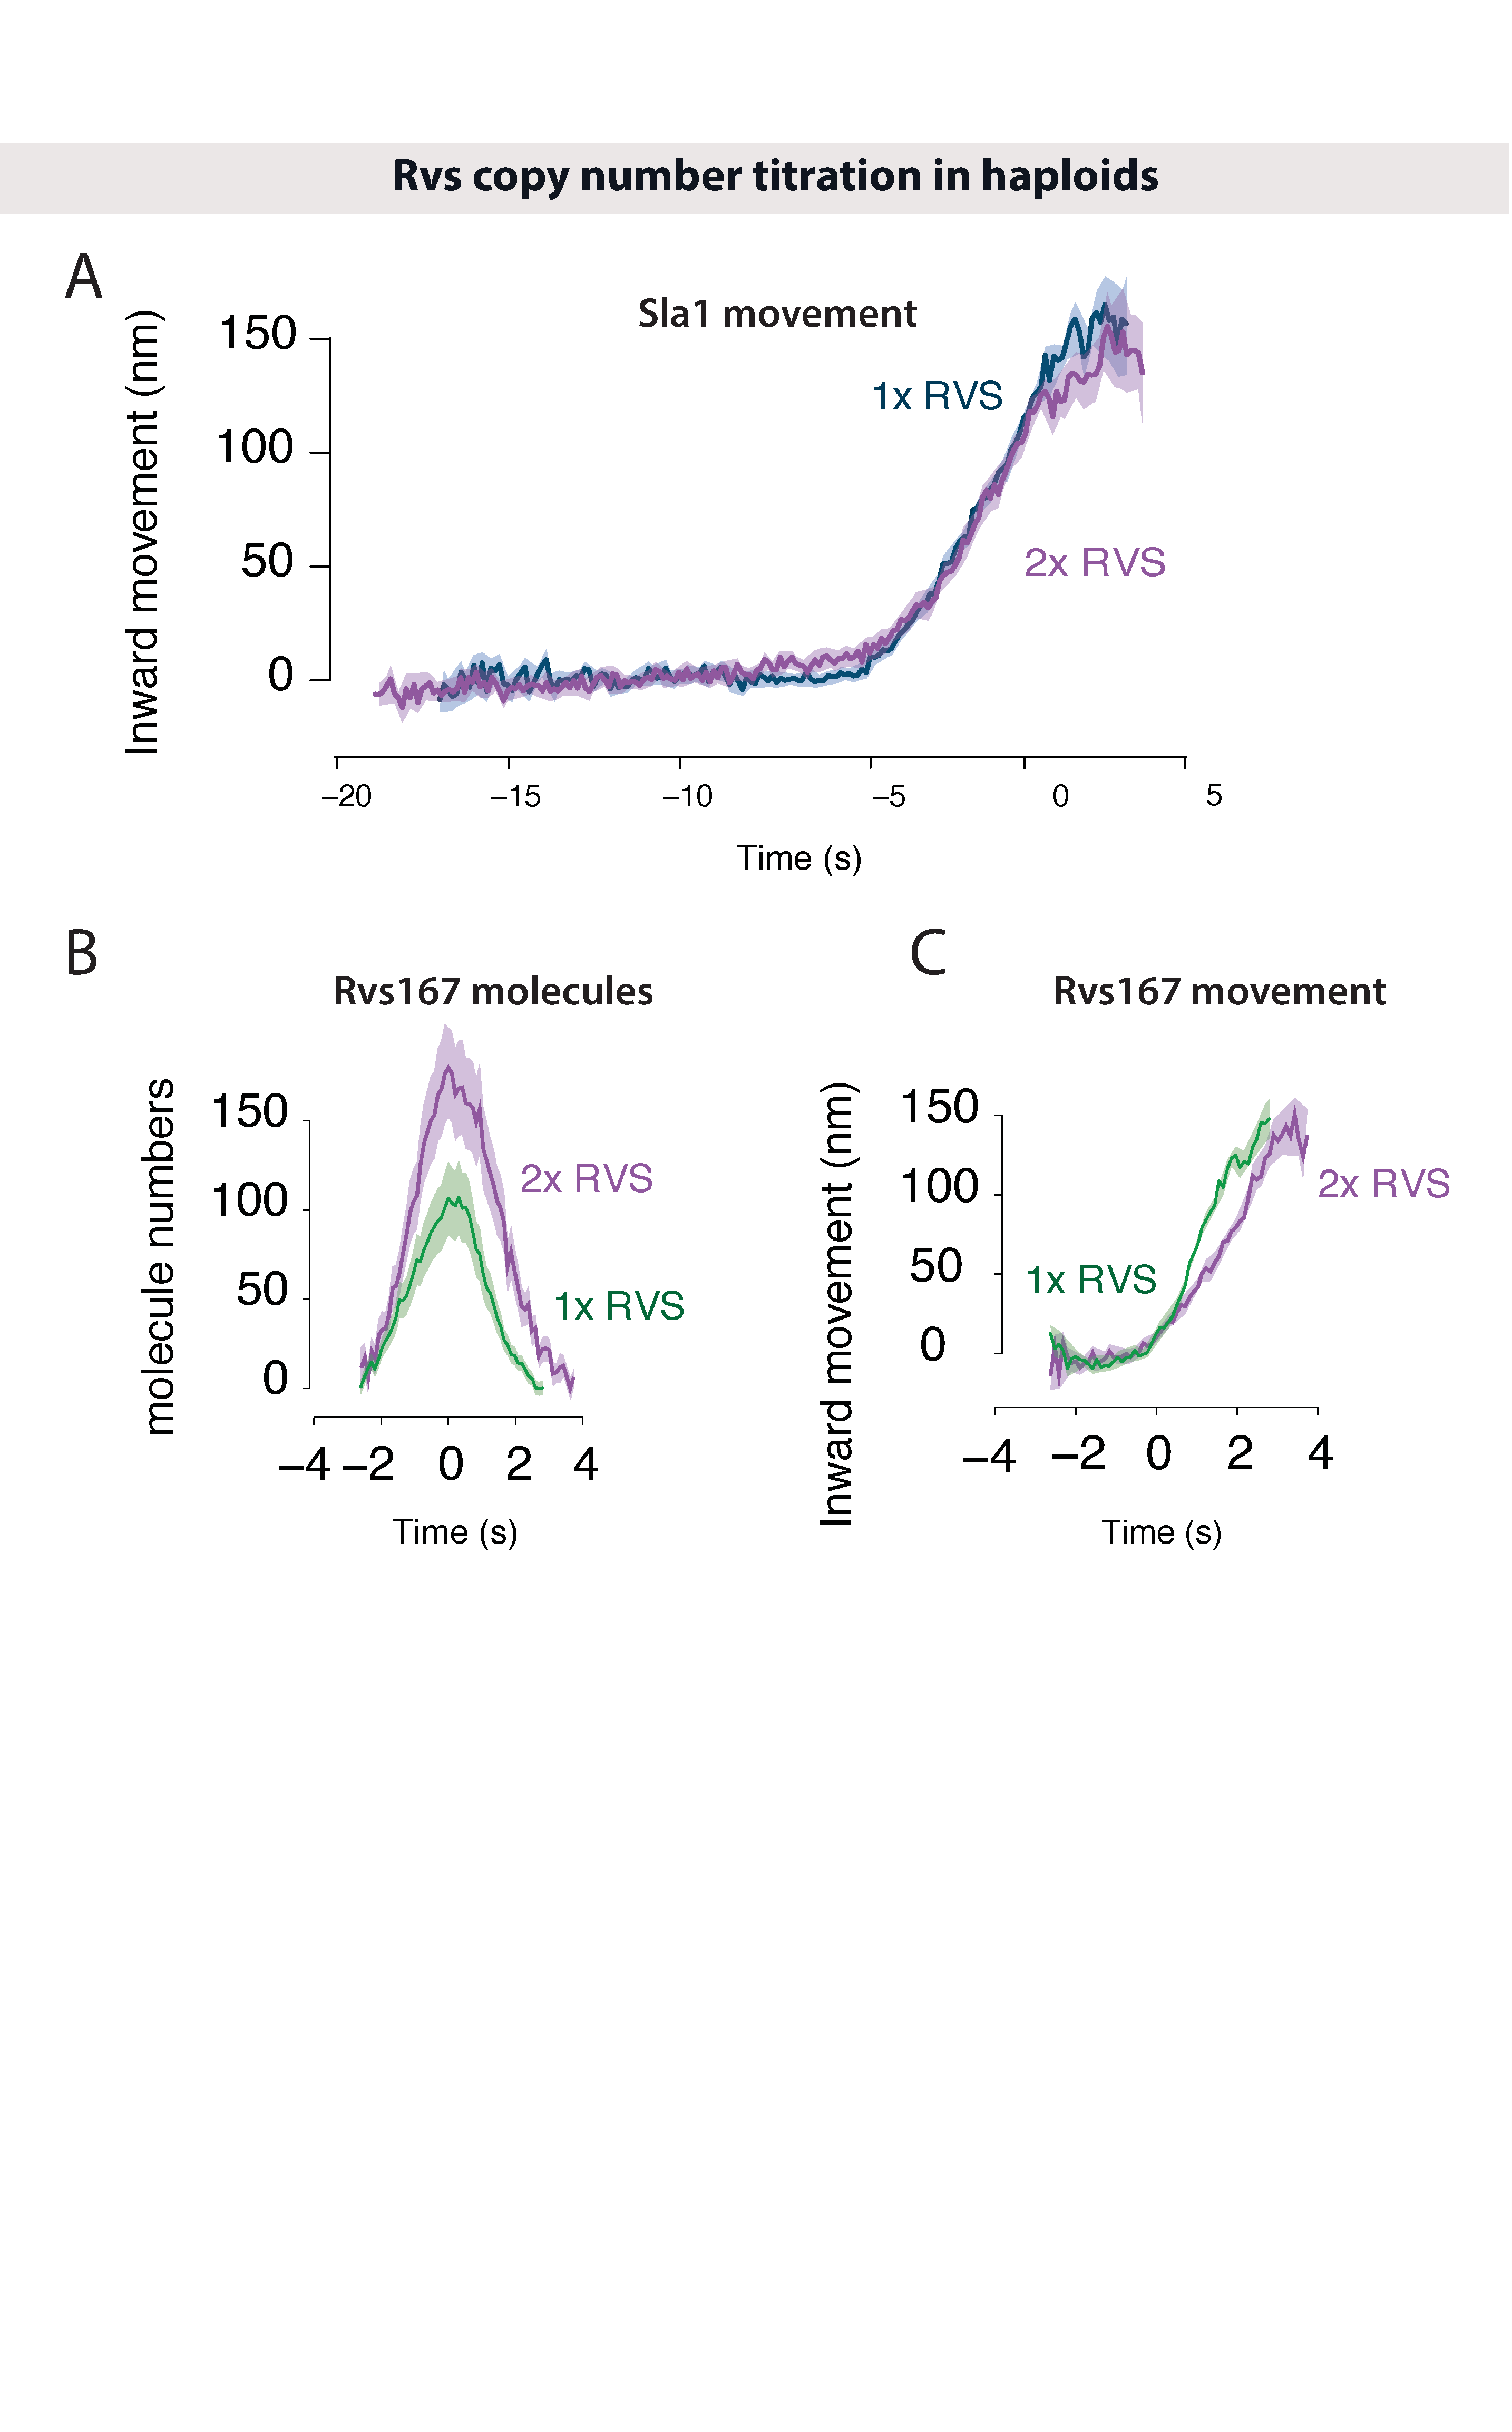
\includegraphics[width=17cm,height=17cm,keepaspectratio]{figures/results_final/rvs_haploid}
		\caption{Sla1 and Rvs167 in Synaptojanin deletion \label{fig5}}
	\end{figure}	

	\vspace{5mm}
	By quantifying the number of Rvs167 proteins as described in Picco et al., 12  first in the haploid strains, I found that in haploids, the average maximum number of Rvs molecules recruited to endocytic sites is 179.7328, SEM=10.1, compared to 113.505, SEM=5.2:  1.6x Rvs is recruited to endocytic sites in the duplicated strain compared to WT. The averaged trajectory of Sla1-GFP, however does not change between the 4x and 2x copies of Rvs: like in the WT, Sla1 moves in to 140nm. The dynamics of Rvs, however is chaged: In Fig.x , the centroid movement of both WT and 2x Rvs167-GFP (henceforth 2x Rvs) is aligned so that time=0 corresponds to the maxima of the fluorescent intensity, which corresponds to scission time. Molecule numbers of 2x Rvs increase at a faster rate than WT, and the disassembly is slowed by ~1 second. In the corresponding Rvs movement trace, instead of the sharp jump seen in WT, there is a delay in the movement into the cytoplasm.


	
	In diploid cells, recruitment of Rvs is similarly measured in the duplicated strain containing 4 copies of both RVS genes (4x Rvs), two copies strain (WT, 2x Rvs), and one copy of each (1x Rvs). Recruitment of Rvs is not directly proportionate to gene copy number: maximum number of Rvs recruited increases from 100.9, SEM=4.6 from in the 2x Rvs strain to 142.5, SEM=5.5 in the 4x strain. In the 1x Rvs strain, 80.2, SEM=4.7 molecules of Rvs are recruited before scission occurs. In order to determine whether this is a reflection on protein availability or if something else limits recruitment of Rvs, I quantified the cytoplasmic intensity of Rvs167-GFP in the respective strains by first producing z-stacks of time-lapse images of cells, and measuring the intensity within the cytoplasm (for details see METHODS). As can be seen in TABLE.X, the number of molecules recruited to endocytic sites scales with the amount of protein in the cytoplasm.  
	\vspace{5mm}
	
	Inward movement of the Rvs centroid is similar for the 4x, 2x and 1x Rvs: the jump inwards is about 80nm. In the 1x strain, however, the centroid disappears immediately after scission, suggesting that there is reduced Rvs at the base of the newly formed vesicle compared to the WT. Recruitment dynamics of all three are different: in the 4x Rvs strain, Rvs is recruited at a rate of 57 molecules/second, which is reduced to 27 molec/sec for the 2x and 19.07 molec/sec for the 1x strain. 

	\vspace{5mm}
	 Sla1 centroid movement, meanwhile is the same in 4x and 2x Rvs strains. In the 1x Rvs strain, Sla1 movement is slightly shifted, suggesting that vesicle scission occurs at invagination lengths about 10nm shorter than that as WT when fewer Rvs molecules are recruited, but increasing Rvs recruitment does not affect membrane progression. 


	
	\subsection{Scission timing is determined by actin forces, \\
		BAR domains prevent scission}
	
	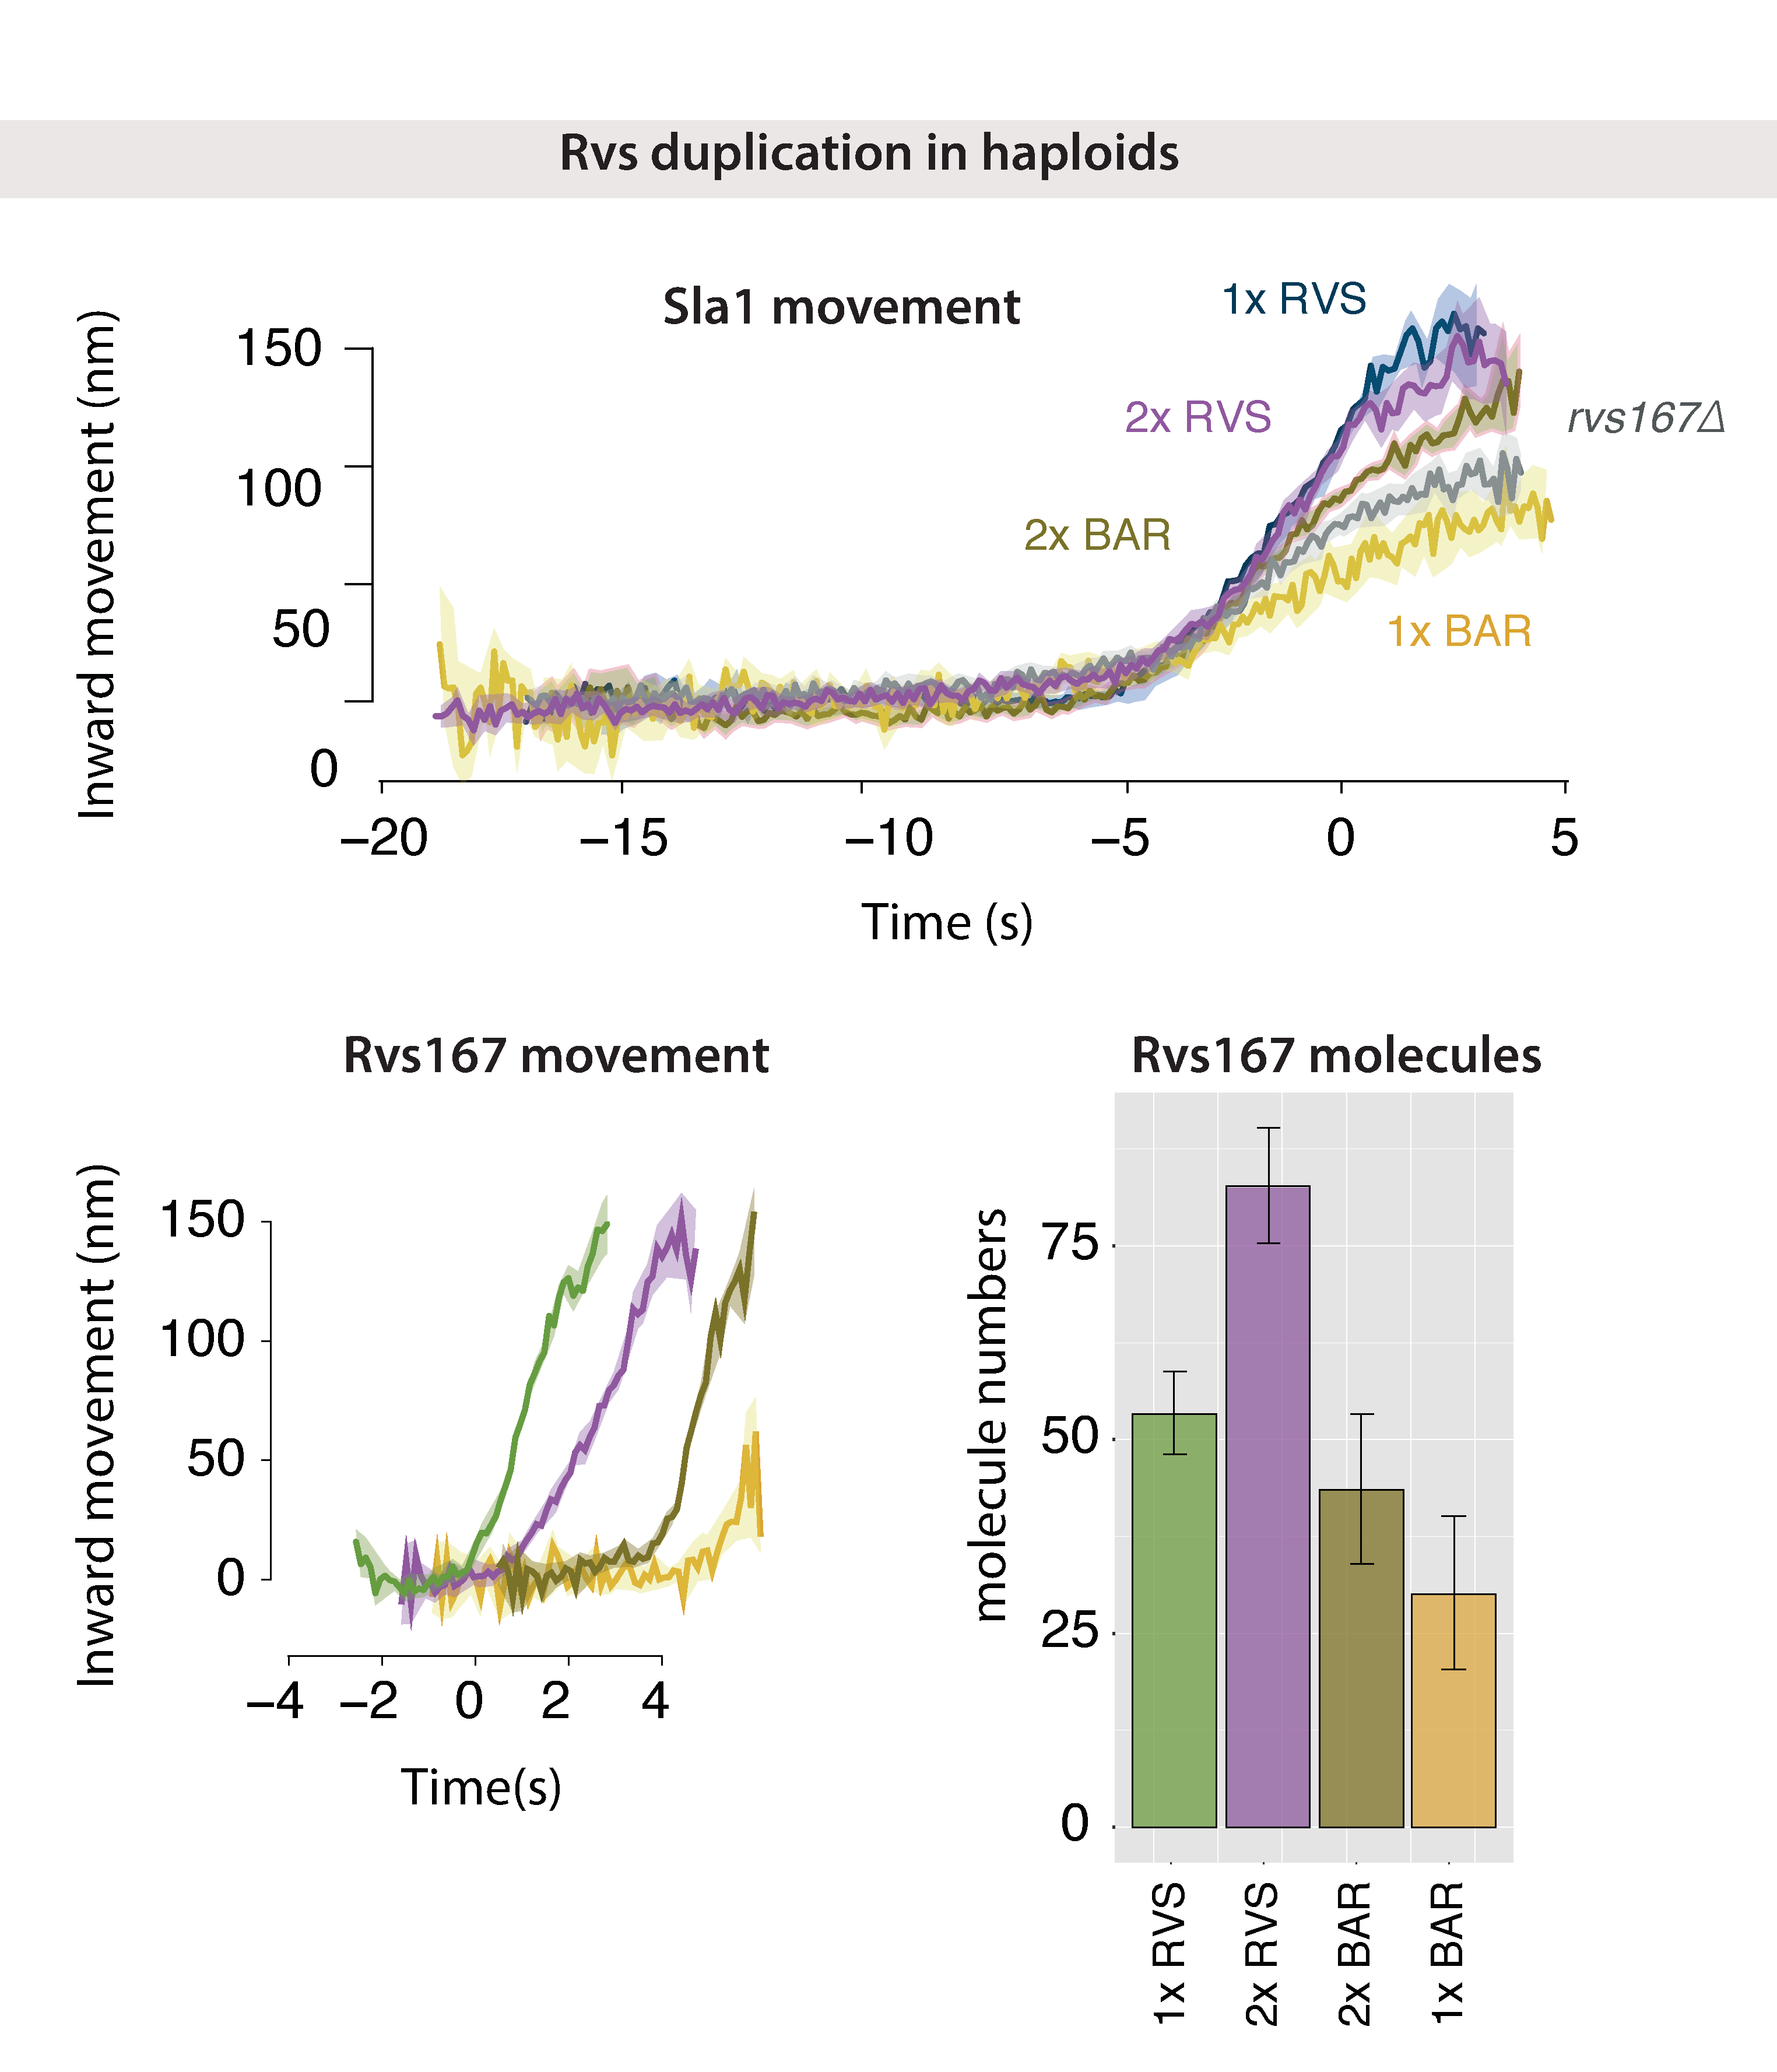
\includegraphics[width=23cm,height=23 cm,keepaspectratio]{figures/results_final/scaffolding}
	
	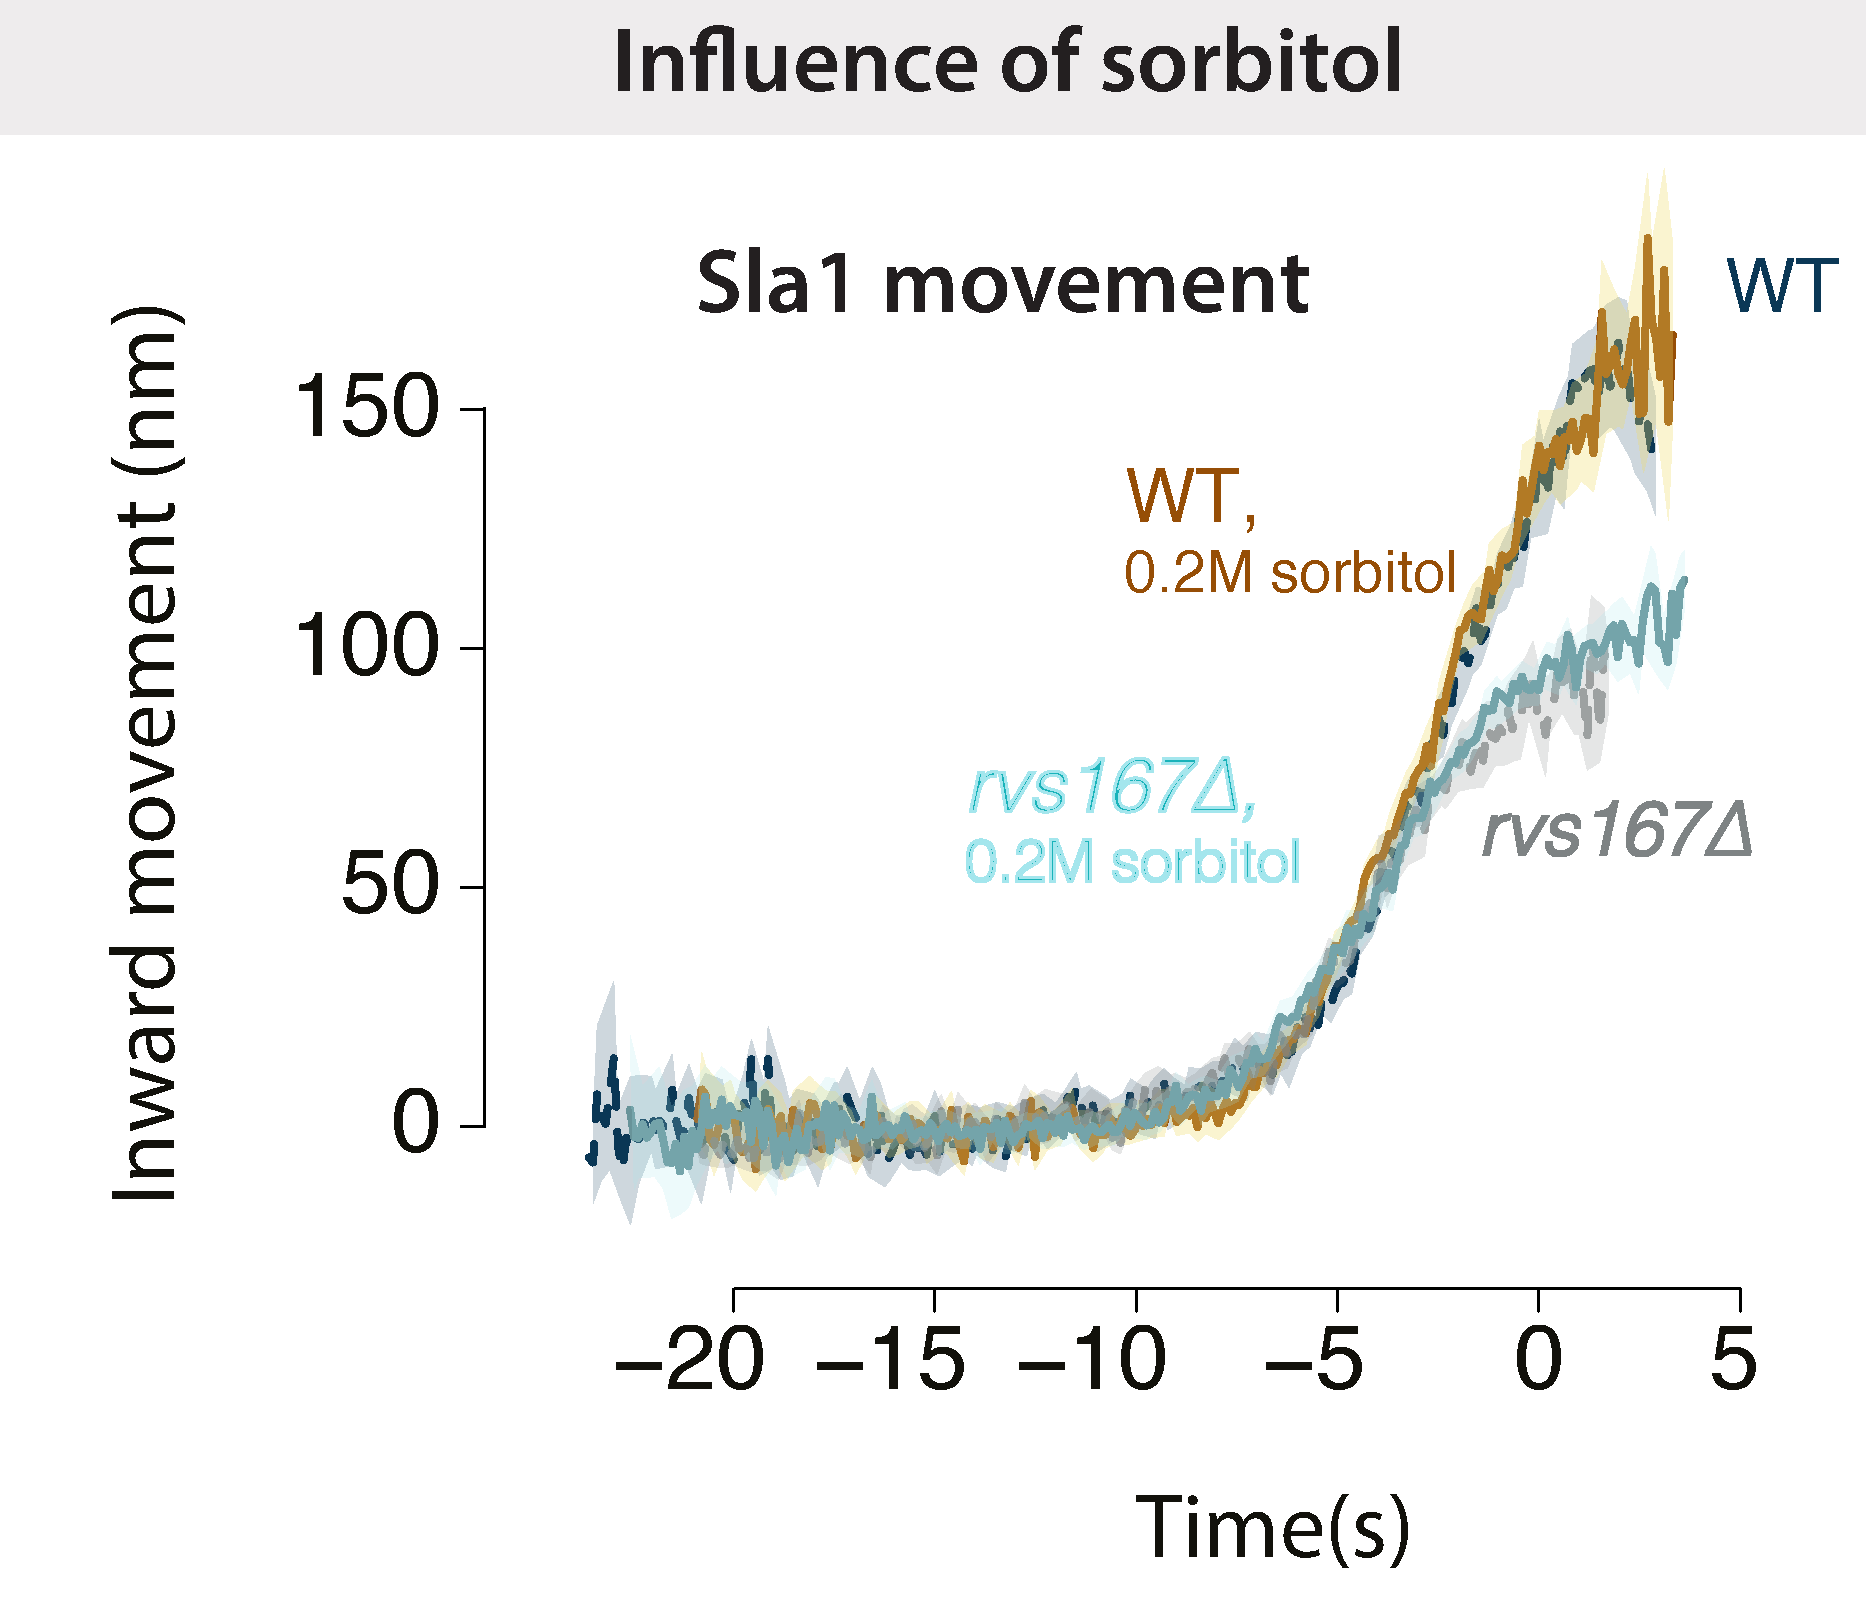
\includegraphics[width=14cm,height=14 cm,keepaspectratio]{figures/results_final/sorbitol}